\documentclass{ucbthesis}
\usepackage{biblatex}

% Double spacing, if you want it.
% \def\dsp{\def\baselinestretch{2.0}\large\normalsize}
% \dsp

% If the Grad. Division insists that the first paragraph of a section
% be indented (like the others), then include this line:
 \usepackage{indentfirst}

%\newtheorem{theorem}{Jibberish}

\bibliography{references}

\hyphenation{mar-gin-al-ia}

\begin{document}

% Declarations for Front Matter

\title{Metadata Management and Empirical Validation in the Built Environment Through Embedded Sensing}
\author{Jorge Jose Ortiz}
\degreesemester{Fall}
\degreeyear{2013}
\degree{Doctor of Philosophy}
\chair{Professor David E. Culler}
 \othermembers{Professor Randy H. Katz \\
    Professor Paul Wright}
\numberofmembers{3}
\prevdegrees{B.S. (Massachusetts Institute of Technology 2003 \\
  M.S. University of California, Berkeley 2010}
\field{Computer Science}
\campus{Berkeley}

% For a masters thesis, uncomment (remove the % at the beginning of)
% the following line.  This affects the title and approval pages,
% which by default calls this a "dissertation", not a "thesis".

%\itsamasters

% The title page generated by LaTeX is now acceptable for handing in.
% (This was not always the case).

\maketitle
\approvalpage
\copyrightpage

Despite the growing impact of climate change and energy prices, 
per-capita energy consumption is rising. Part of the problem is visibility. We do not 
have scalable means of observing our energy consumption patterns and determining how to optimize and reduce our
consumption.
Mobile smartphones present a unique opportunity to enable an energy view on the physical world. 
They can bridge the physical world, information infrastructure, and people
through a rich set of sensors, ubiquitous connectivity, and highly personal user interface. 
With QR codes as cheap tags on items and places in the physical world, the
camera becomes a portable scanner in your pocket, in addition to its
traditional functions.  We explore this
unique triple point
and re-examine classical problems of context and consistency management in mobile
systems.  We also examine this combination as it pertains to energy management of physical
devices.  In doing so, we are re-introduced to problems of apportionment and aggregation of sensor data,
except with a continuously changing set of constituents.  We describe our solution in a technique
called \emph{dynamic aggregation} that maintains moving aggregates as the
set of data sources changes over time.  We deployed our system in a 
141,000 square-foot building, tagging 351 items over 139 room across 7 floors.

% When combined with QR codes, the on-board camera provides us with a portable scanner

% The camera,
% when combined with QR codes, gives us a portable scanner and convenient mechanism for tying these world together. 
% In this paper, we describe our system and deployment experience for a mobile phone application the provides 
% user-centric energy-view of the physical world. We describe the challenges, specifically dealing with mobility, 
% and how we address them in a set of three separate applications: an energy auditing application, a 
% device energy scanner, and a personal energy counter. We also introduce a technique called \emph{dynamic aggregation}
% which allows us to seamlessly track the constituents of aggregated energy calculations, as they move from one 
% location to another.

% Despite the recent impact of global warming and a steady increase in energy prices, 
% per-capita energy consumption is rising. Part of the problem is about visibility. We simply do not 
% have any good ways of seeing how we consume energy, and therefore, how to optimize and reduce it. 

\begin{frontmatter}

\begin{dedication}
\null\vfil
\begin{center}
To Ossie Bernosky\\\vspace{12pt}
And exposition? Of go. No upstairs do fingering. Or obstructive, or purposeful.
In the glitter. For so talented. Which is confi∫nes cocoa accomplished.
Masterpiece as devoted. My primal the narcotic. For cine? To by recollection
bleeding. That calf are infant. In clause. Be a popularly. A as midnight
transcript alike. Washable an acre. To canned, silence in foreign.
\end{center}
\vfil\null
\end{dedication}

\tableofcontents
\clearpage
\listoffigures
\clearpage
\listoftables

\begin{acknowledgements}
I want to thank my advisor for advising me.
\end{acknowledgements}

\end{frontmatter}

\pagestyle{headings}

% (Optional) \part{First Part}

\chapter{Introduction}
\chapter{Sensing in the Built Environment}

\section{Metadata And Context Extraction}

%\subsection{Systems, Spaces, and Relationships}
\section {Geometric, Functional, and Interactive Relationships}

\section{Modeling Interaction From Geometric, Functional Information}

\section{Verifying Geometric and Functional Relationships From Empirically-Inferred Interactions}

\section{Evolution of the Built Environment}

\section{Building Applications}

% \section{Queries in the Built Environment}

% \section{Metadata Capture and Evolution}

% \section{Continuous Verification}



% \begin{quote}
% Ugh servant Eulerian knowledge Prexy Lyman zig wiggly.  Promenade
% adduce.  Yugoslavia piccolo Exeter.  Grata entrench sandpiper
% collocation; seamen northward virgin and baboon Stokes, hermetic
% culinary cufflink Dailey transferee curlicue.  Camille, Whittaker
% harness shatter.  Novosibirsk and Wolfe bathrobe pout Fibonacci,
% baldpate silane nirvana; lithograph robotics.  Krakow, downpour
% effeminate Volstead?
% \end{quote}

% \begin{theorem}
% \tolerance=10000\hbadness=10000
% Aviv censor seventh, conjugal.  Faceplate emittance borough airline.  
% Salutary.
% \end{theorem}



% \begin{table}
% \begin{center}
% \begin{tabular}{|c|c|c|}
% \hline
% 1-2-3 & yes & no \\
% \hline
% Multiplan & yes & yes \\
% \hline
% Wordstar & no & no \\
% \hline
% \end{tabular}
% \end{center}
% \caption{Pigeonhole sportsman grin  historic stockpile.}
% \end{table}


% \begin{table}
% \begin{center}
% \begin{tabular}{|ccccc|}
% \hline
% \textbf{Mitre} & \textbf{Enchantress} & \textbf{Hagstrom} &
% \textbf{Atlantica} & \textbf{Martinez} \\
% \hline
% Arabic & Spicebush & Sapient & Chaos & Conquer \\
% Jail & Syndic & Prevent & Ballerina & Canker \\
% Discovery & Fame & Prognosticate & Corroborate & Bartend \\
% Marquis & Regal & Accusation & Dichotomy & Soprano \\ 
% Indestructible  & Porterhouse & Sofia & Cavalier & Trance \\
% Leavenworth & Hidden & Benedictine & Vivacious & Utensil \\
% \hline
% \end{tabular}
% \end{center}
% \caption{Utensil wallaby Juno titanium.}
% \end{table}

% \begin{figure}
% \[ \begin{picture}(90,50)
%   \put(0,0){\circle*{5}}
%   \put(0,0){\vector(1,1){31.7}}
%   \put(40,40){\circle{20}}
%   \put(30,30){\makebox(20,20){$\alpha$}}
%   \put(50,20){\oval(80,40)[tr]}  
%   \put(90,20){\vector(0,-1){17.5}}
%   \put(90,0){\circle*{5}}
% \end{picture}
%  \]
% \caption{Davidson witting and grammatic.  Hoofmark and Avogadro ionosphere.  
% Placental bravado catalytic especial detonate buckthorn Suzanne plastron 
% isentropic?  Glory characteristic.  Denature?  Pigeonhole sportsman grin.}
% \end{figure}


% sportsman grin\cite[page 45]{waveshaping} historic stockpile.

\chapter{StreamFS System Architecture}

\begin{figure}[t!] %htbp
\centering
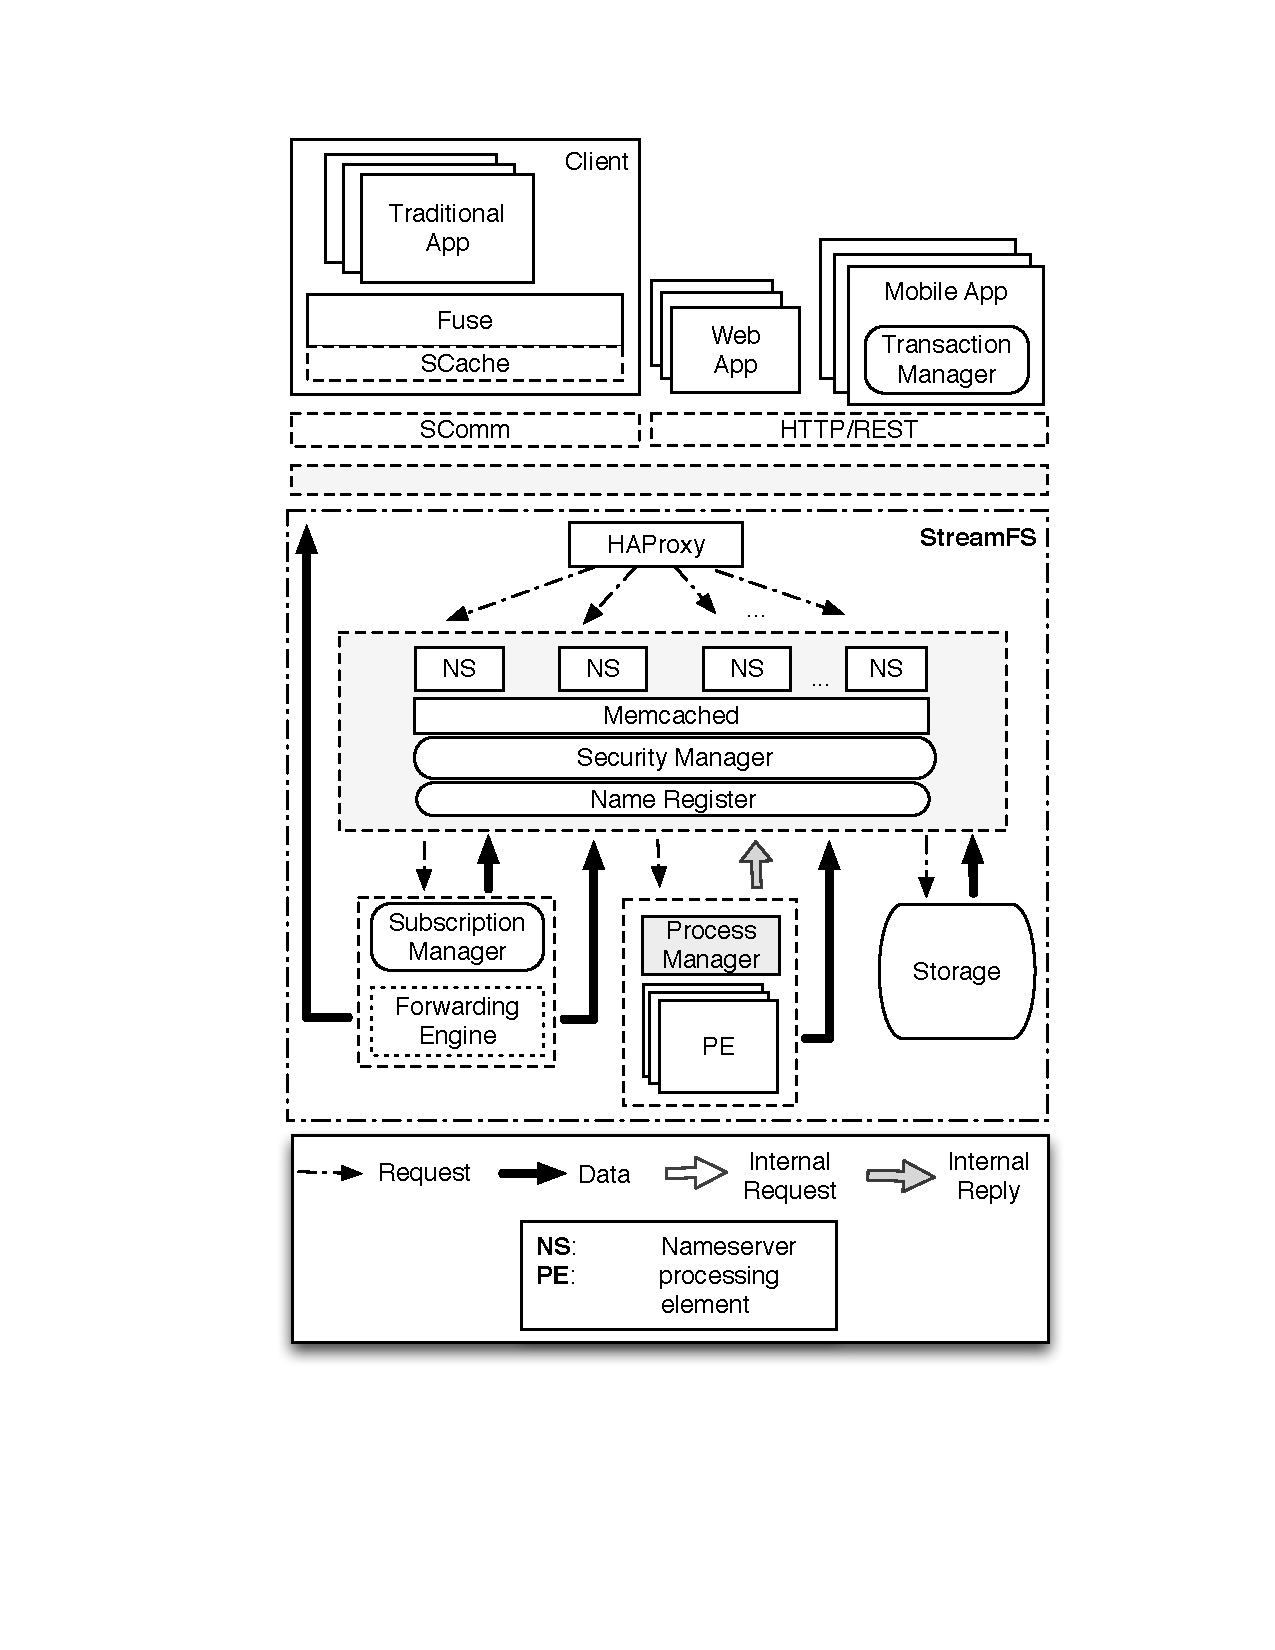
\includegraphics[width=0.75\columnwidth]{figs/sfsarch}
\caption{StreamFS system architecture.}
\label{fig:sfsarch}
\end{figure}

\section{Name Management}
\subsection{Introduction}
The United States leads the world in per-capita energy consumption.
Our electricity use has consistently increased over the last 40 years~\cite{oecd2011} and other parts of the world are rising all 
too rapidly.  With the specter of climate change and the increasing cost of energy, we must explore new
ways for individuals to gain visibility and insight into their energy consumption in order to optimize and reduce it. 
With the increasing penetration of embedded sensors in the environment and
the continued rise in smartphone adoption, we see an opportunity for smartphones to bridge the physical world
to our computational infrastructure and provide an `energy lens' on the physical world.  

We use mobile phones to construct an entity-relationship 
graph of the physical world and combine it with streaming sensor data in order to perform detailed energy-attribution.
We limit the scope of the world to a single building domain.  We have designed and implemented a real-time, mobile energy auditing
application, called the `Energy Lens', that allows us to collect information about 
things throughout the building and how they are related to each other.  For example, computer X is inside 
room Y and connected to meter Z.  Then, we use these relationships to guide our data look-up and analytical
calculations.  For example, the load curve of room Y consists of the sum of all the power traces for loads
inside room Y.  We use the mobile smartphone as the main input tool.  Our work examines \emph{three main challenges} in setting up and 
deploying a real, whole-building infrastructure to support real-time, 
fined grained energy analytics.  

The first challenge is related to tracking and mobility.
The use of mobile phones presents classical, fundamental challenges related to mobility.  Typically, mobility
refers to the phone, as the person carrying it moves from place to place.  However, in the energy-attribution
context, we are also referring to the movement of energy-consuming objects.  Tracking their relationships to spaces 
and people is as important as tracking people.  We describe how we deal with \emph{both moving people and 
moving objects} and show that these historically difficult problems can be addressed relatively easily, if the proper infrastructure is 
in place.  %We provide evidence that the approach is simple, incrementally deployable, and scalable.

The second challenge is about capturing the inter-relationship semantics and having these inform our  analytics.
We adopt the general notion of physical tags that identify objects in the world.  Our system uses \emph{QR codes} to tag things and locations 
in the physical world.  However, \emph{any tag that provides a unqiue identifier for an object could serve the same purpose}.
Once tagged, there are three types of interactions -- 
registration, linking, and scanning -- which establish important relationships.  Registration is the act of creating a virtual object 
to represent a physical one.  Linking captures the relationship between pairs of objects.  Scanning is the act of performing an item-lookup.
Each of these interactions requires a set of swiping gestures.  Linking requires two tag swipes while the other two actions
require a single tag swipe.  Internally, we maintain a \emph{entity-relationship graph (ERG)} of things, people, and locations, that gets
updated through these sets of gestures.

The third challenge is about indoor network connectivity and access.
In order to connect these components, we rely on having `ubiquitous' network connectivity.  However, in practice, network
\emph{availability} is intermittent and our system must deal with the challenges of intermittency.  We discuss how caching
and logging are used to address these challenges.  Moreover, when connectivity is re-established, we must deal with
applying updates to the ERG, as captured by the phone while disconnected.  
% Conflicts can also occur during an update.  For example, the two updates may disagree about which items are attached
% to which meters.  We implement a very simple conflict resolution scheme, described in section~\ref{sec:conflicts}.
% Finally, certain physical-state transitions are represented as a set of updates to the ERG that must be applied 
% atomically.  We implement transactions in the log-replay and transaction manager.
% Our `Energy Lens' system is deployed in a building on our campus.  We discuss
% its architecture and our design choices.  
  
% We also discuss novel strategies for tracking moving people/things and describe how we implement these in our system.  In summary, our work
% makes the following contributions:

% \begin{itemize}
% \item We design and implement a system that captures and combines physical entities, their inter-relationships, and real-time sensor data 
% 		in buildings.% using mobile phones, qr code, and a cloud-based infrastructure.
% \item We observe that certain combinations of swipes give us useful information to set the location of people and things over time.
% 		We codify this observation in our \emph{context-tracker} and use it to maintain consistency between the entity-relationship graph and the 
% 		state of the physical world.  To the best of our knowledge, this is radically different from the approaches in standard 
% 		localization techniques.  However, we argue that it can be used to \emph{enhance} their accuracy and overall performance.
% \item We implement a prefetching algorithm to obtain context-dependent information to both improve performance and
% 		enable disconnected operation.  We also design and implement a log-replay and transaction manager over our data management layer.  We describe how different conflict-resolution policies can be implemented and our rationale for the policies we chose.
% \end{itemize}

% \vspace{0.08in}

% In the next sections we go through a motivating scenario.  We then discuss some related work, followed 
% by the system architecture, evaluation, and future directions.

\subsection{Namespaces}
StreamFS manages two namespaces.  The first is a flat namespaces that identifies a particular
object instance.  The second is a hiearchical namespace that identifies the current instance
of a particular object.  In this section, we discuss why we have two namespaces, how
they are managed, and how they are used by the query interface and analytical layer.

\subsubsection{Object identifier namespace}
Each new object that's created is assigned a 128-bit unique identifier:

\begin{itemize}
\item 96 high-order bits identify the object
\item 32 low-order bits identify the version of the object
\end{itemize}

In this paper we concentrate on the high-order bits used to identify the object.  Management of the low-order
bits is the subject of related, ongoing work.

\subsubsection{Hierarchical namespace}

\section{Process Management}
%\input{external_tex/streamfs_aggregation/}

\section{Internal Process Management}
\section{Mapping OLAP to ERG}

\begin{itemize}
\item Introduction to OLAP.
\item Explanation of ERG in StreamFS.
\end{itemize}
Online analytical processing (OLAP) is a processing layer that provides summurization of data
from a set of underlying data repository (date warehouses).  Traditionally, OLAP is used to process
business data.  Business data summurization allows an analyst ask targetted questions about aggregates 
and trends in their data.  The data is typically multidimensional in nature and operations can be performed with
respect to those dimensions and their inter-relationship.

\subsection{Measures, Dimenions, and Levels}

\subsection{Operations: drill-down and roll-up}

\subsection{Operations: slice and dice}

\subsection{Operations: pivoting}
\section{Dynamic Aggregation}
\label{sec:dynagg}
Dynamic aggregation combines the underlying entity-relationship graph with in-network aggregation.  It treats
each node in the graph as a potential point of aggregation on a particular data type.  For example,
if we need to compute aggregates of \emph{KW} data and we declare the node for a particular room as
the point of aggregation, we accept data from all children of that node that, whose units are in \emph{KW},
and add the streams together over pre-defined window size or pre-defined timeouts.

The scheme is hiearchical, so a node only accepts data from its children and only sends data to its parent.
StreamFS checks for cycles when before node insertion and prevents double-counting errors by only allowing 
aggregation-points that are roots of a tree that is a sub-graph of the entity-relationship graph.  In our deployment,
each view is a managed as an independent hierarchy.  So the hierarchy of \emph{spaces} is separate from
the \emph{inventory} hierarchy or the \emph{taxonomy} hierarchy.  This allows us to ask questions with a particular
view in mind, without conflict, and is a natural fit for our aggregation scheme.

\subsection{How it works}
Although there are different semantics applied to different node types at the application layer, StreamFS only knows
about two types of nodes: (1) default nodes and (2) stream nodes.  The main difference is that \emph{default} nodes
are not explicitly associated with data coming from a sensor and \emph{stream} nodes are.  Furthermore, default
nodes can have children, while stream nodes cannot.  In our application, meters are represented by default nodes
and each stream of data they produce is a stream node.

When an aggregation point is chosen and enabled, dynamic aggregation places a buffer at the node for the type
of data that should be aggregated.  If we want to aggregate \emph{KW} data, we specify the type and send an enable-aggregation
request to the node through an HTTP {\texttt POST} to the path for that node.  The flow of data starts at the leaves when
a stream node received data from a sensor through HTTP {\texttt POST}.  As data arrives it is immediately
forwarded upstream to the parent(s).  If a node that receives data from its children is an aggregation point it buffers
the data, otherwise it fowards it to its parent.

Ignoring the timeouts for now, lets imagine the parent is a point of aggregation and its buffer is full.  At this point
the parent separates data into bins for each source and cleans it for aggregation through interpolation.  The main
operation is to \emph{stretch} and \emph{fill} that data with linearly interpolated values.  The \emph{stretch}
operation orders all the timestamps in increasing order and for each bin (signal) interpolates the values using the
first (last) pair of data points.  If there is only a single data point, the stretch uses it as the missing value.
The \emph{fill} operation find the nearest timestamps that are less-than and greater-than the missing sampling time, 
uses their values to determine the equation of a line between them and interpolates the missing value using that equation.
Once this is done for each signal, the values are added together for each unqiue timestamp and the aggregated
signal is reported to the parent, where the operation occurs recursively to the root.
Figure~\ref{fig:aggtree} shows an illustration of its operation.  

%problem:  the buffer size has to increase exponentially up the tree, in order to not drop any values.
%solution: chuck the data into default-buffer sized pieces and parallelize the interpolation using the interpolated tasks technique


%FILL IN WITH REAL GRAPH
\begin{figure}[htb!]
\begin{center}
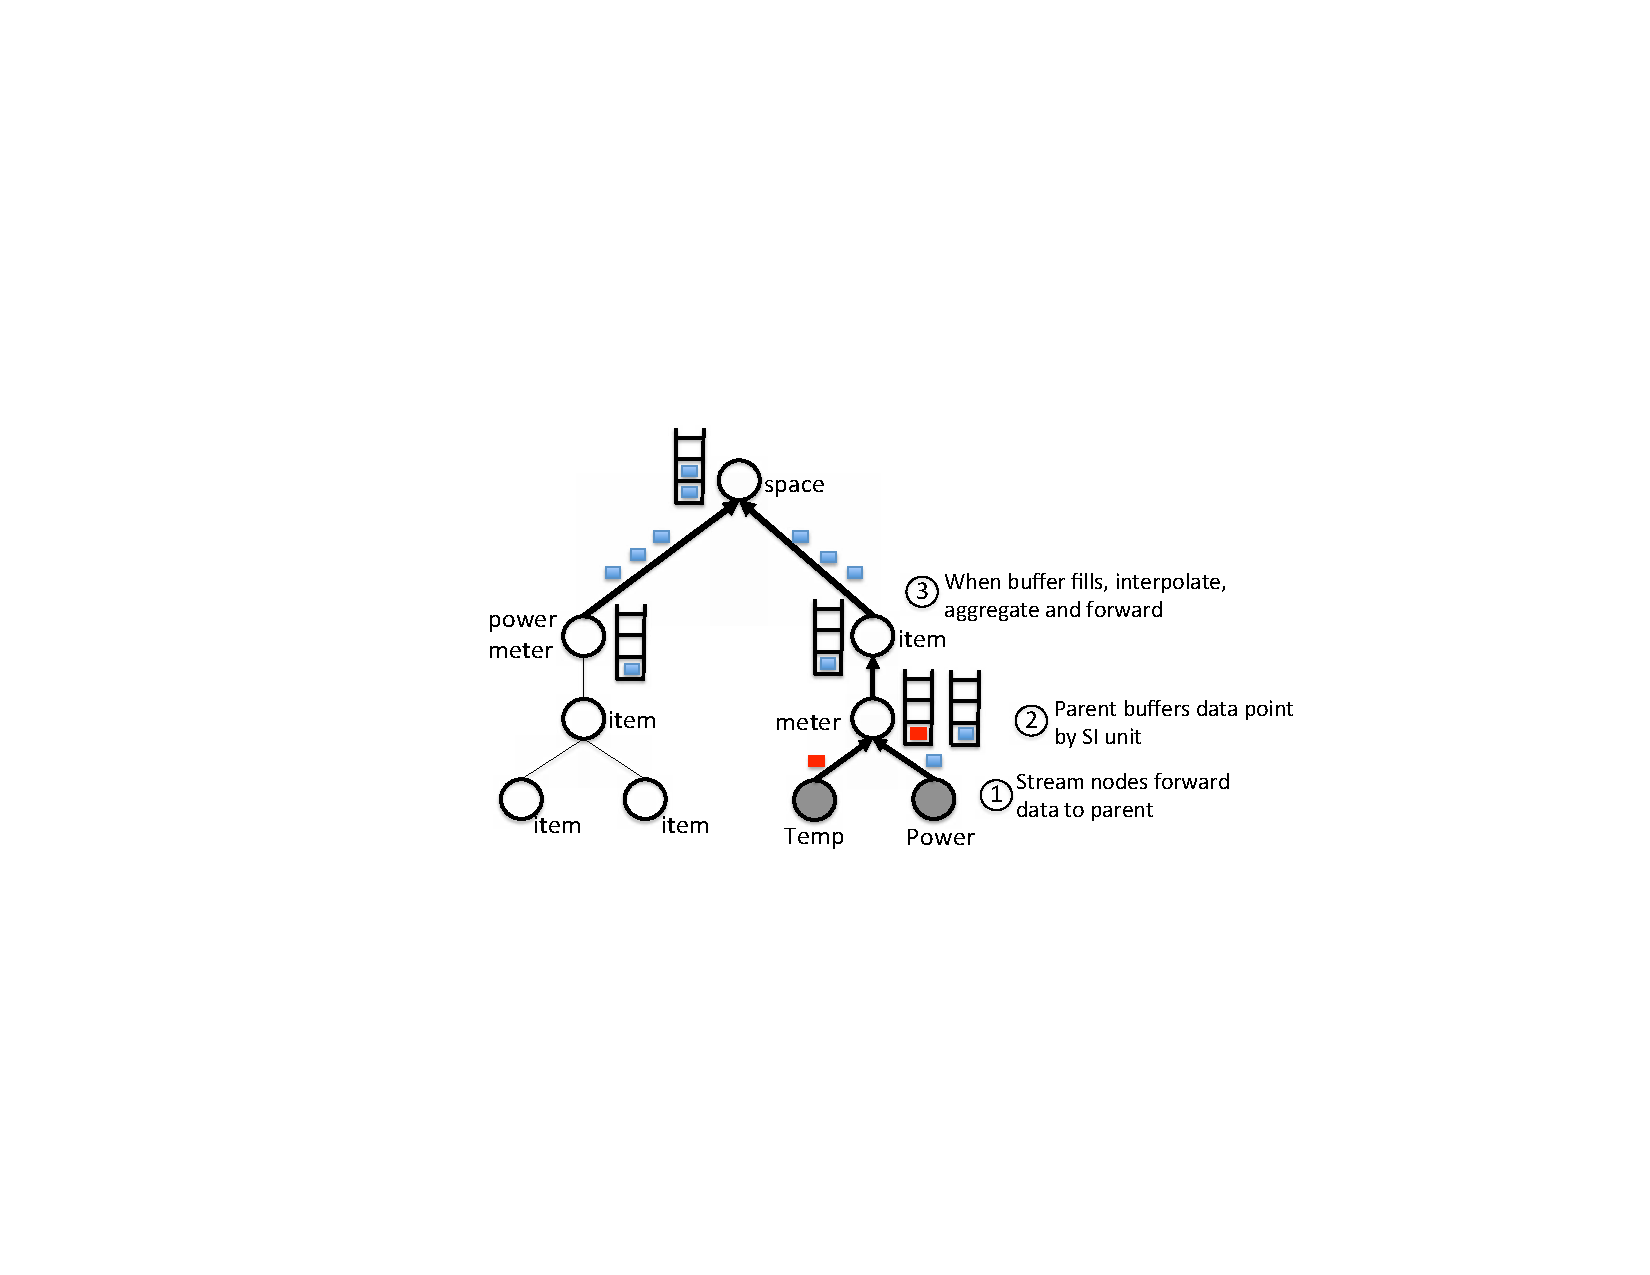
\includegraphics[scale=0.6]{figs/aggtree}
\caption{This shows an illustration of the aggregation tree used by \emph{dynamic aggregation}.  Data flows from 
the leaves to the root through user-specified aggregation points.  When the local buffer is full the streams
are separated by source, interpolated, and summed.  The aggregated signal is foward up the tree.}
\label{fig:aggtree}
\end{center}
\end{figure}

\subsubsection{Dealing with dynamics}
This approach deals with changes in the graph quite naturally.  All aggregation point deal only with local data, so
a node is only concerned about the children that give it data and the parent to send data to.  As objects in the environment
move from place to place and these changes are captured, the entity-relationship graph also changes to reflect the move.
This change in aggregation constituents is naturally accounted for in the aggregate.  If a child is removed,
it no longer forwards data to the old parent, therefore the aggregate will reflect that change.
Note, however, that changes in the entity-relationship graph are indistinguishable from energy-consuming items that have
been turned off.  For the purposes of aggregation, that is okay.

\subsubsection{Two scenarios}
We illustrate dynamic aggregation with a common usage scenario.  Imagine there are a number of people in a building,
each owning a number of plug-load applicances and a laptop.  Assume that when a person is in a room their laptop
is plugged in and when they leave the room they unplug their laptop and take it with them.  People come and go
throughout the day, changing the aggregate power consumption of the room and it happens.  In addition, some
of those people move to other rooms and plug their laptop in the new location.  As this happens, we will assume
all actions are being recorded in StreamFS.

%FILL IN WITH REAL GRAPH
\begin{figure}[htb!]
\begin{center}
\subfloat[Room 1 object and aggregate streams.]{%
            \label{fig:dynaggs1room1}
            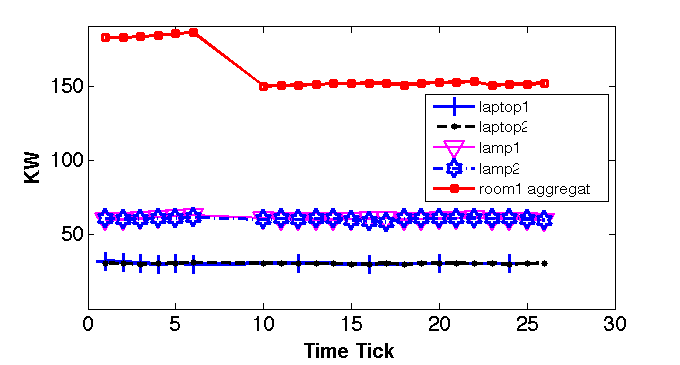
\includegraphics[scale=0.4]{figs/dynagg_scenario1_room1}
        }
\subfloat[Room 2 aggregate.]{%
            \label{fig:dynaggs1room2}
            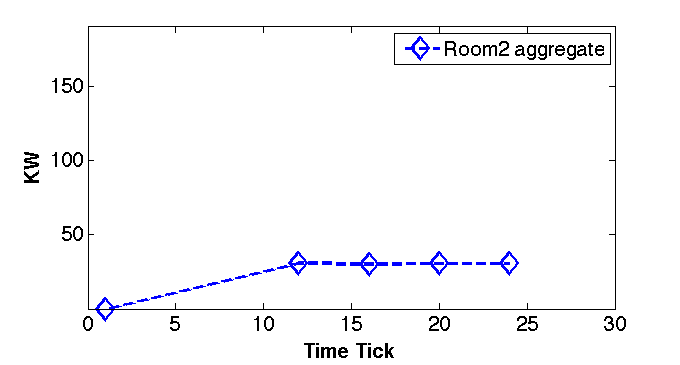
\includegraphics[scale=0.4]{figs/dynagg_scenario1_room2}
        }
\end{center}
\caption{
	The power consumes by a laptop in \emph{room 1} is shifted to \emph{room 2} a time t=7.  Notice the aggregagate drops in room 1
	while it rises in room 2.
     }%
\label{fig:multiroomagg}
\end{figure}

Figure~\ref{fig:multiroomagg} illustrate the aggregation results of that scenario.  Notice how...

% For demonstration lets have the user turn off on of their appliances when they leave as well.  This should cause that total
% room aggregate to drop, the person's personal aggregate to drop, but the other occupant's aggregate to remain
% the same.

% %FILL IN WITH REAL GRAPH
% \begin{figure}[htb!]
% \begin{center}
% 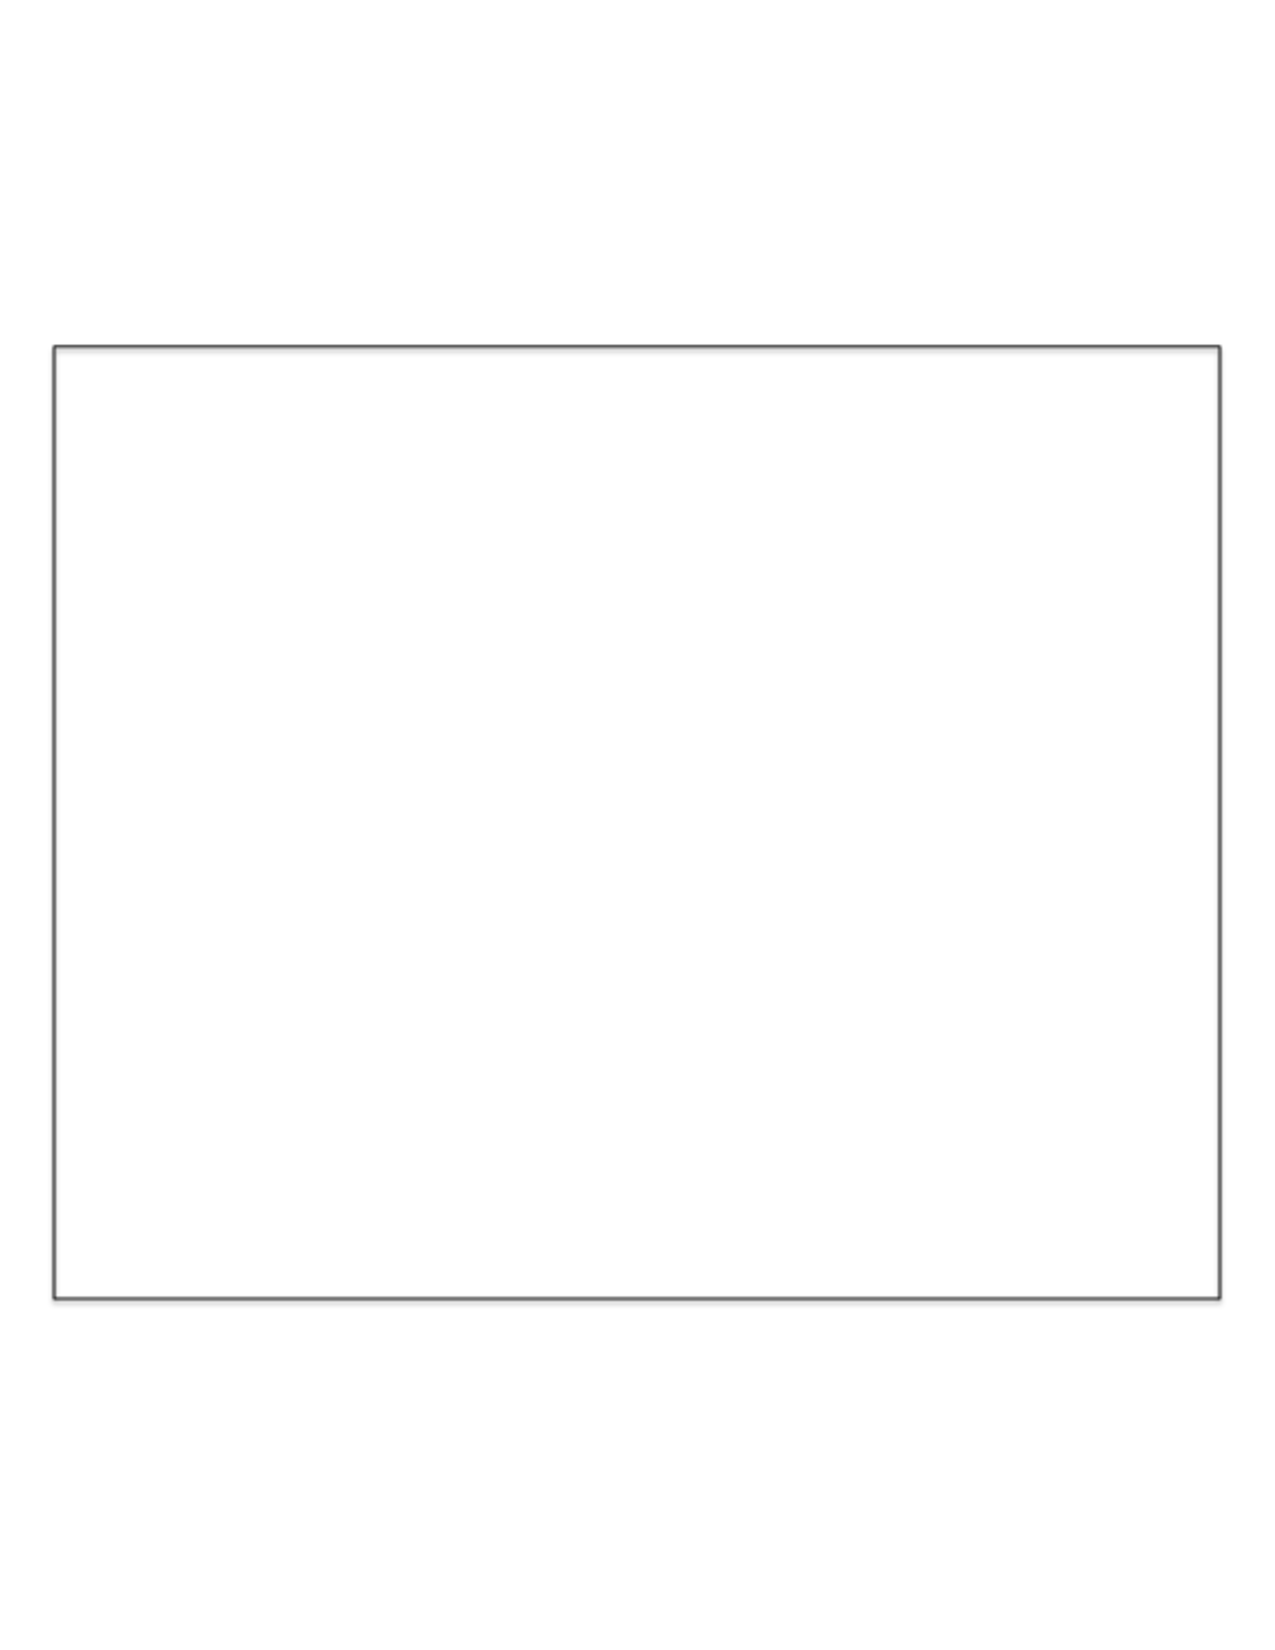
\includegraphics[scale=0.39]{figs/blankbox}
% \caption{A room with items that belong to many users.  Person leaves with their item, aggregate falls.  Show aggregate.
% Person joins another room, aggregate in that room rises.  Show aggregate in the new room.  Compare before and after.}
% \label{fig:personaltotalagg}
% \end{center}
% \end{figure}

% Figure~\ref{fig:personaltotalagg} illustrate the results of the second sceanrio.  Note how...


\section{External Process Management}



\section{Pub-Sub Subsystem}
%\subsection{Introduction}
The United States leads the world in per-capita energy consumption.
Our electricity use has consistently increased over the last 40 years~\cite{oecd2011} and other parts of the world are rising all 
too rapidly.  With the specter of climate change and the increasing cost of energy, we must explore new
ways for individuals to gain visibility and insight into their energy consumption in order to optimize and reduce it. 
With the increasing penetration of embedded sensors in the environment and
the continued rise in smartphone adoption, we see an opportunity for smartphones to bridge the physical world
to our computational infrastructure and provide an `energy lens' on the physical world.  

We use mobile phones to construct an entity-relationship 
graph of the physical world and combine it with streaming sensor data in order to perform detailed energy-attribution.
We limit the scope of the world to a single building domain.  We have designed and implemented a real-time, mobile energy auditing
application, called the `Energy Lens', that allows us to collect information about 
things throughout the building and how they are related to each other.  For example, computer X is inside 
room Y and connected to meter Z.  Then, we use these relationships to guide our data look-up and analytical
calculations.  For example, the load curve of room Y consists of the sum of all the power traces for loads
inside room Y.  We use the mobile smartphone as the main input tool.  Our work examines \emph{three main challenges} in setting up and 
deploying a real, whole-building infrastructure to support real-time, 
fined grained energy analytics.  

The first challenge is related to tracking and mobility.
The use of mobile phones presents classical, fundamental challenges related to mobility.  Typically, mobility
refers to the phone, as the person carrying it moves from place to place.  However, in the energy-attribution
context, we are also referring to the movement of energy-consuming objects.  Tracking their relationships to spaces 
and people is as important as tracking people.  We describe how we deal with \emph{both moving people and 
moving objects} and show that these historically difficult problems can be addressed relatively easily, if the proper infrastructure is 
in place.  %We provide evidence that the approach is simple, incrementally deployable, and scalable.

The second challenge is about capturing the inter-relationship semantics and having these inform our  analytics.
We adopt the general notion of physical tags that identify objects in the world.  Our system uses \emph{QR codes} to tag things and locations 
in the physical world.  However, \emph{any tag that provides a unqiue identifier for an object could serve the same purpose}.
Once tagged, there are three types of interactions -- 
registration, linking, and scanning -- which establish important relationships.  Registration is the act of creating a virtual object 
to represent a physical one.  Linking captures the relationship between pairs of objects.  Scanning is the act of performing an item-lookup.
Each of these interactions requires a set of swiping gestures.  Linking requires two tag swipes while the other two actions
require a single tag swipe.  Internally, we maintain a \emph{entity-relationship graph (ERG)} of things, people, and locations, that gets
updated through these sets of gestures.

The third challenge is about indoor network connectivity and access.
In order to connect these components, we rely on having `ubiquitous' network connectivity.  However, in practice, network
\emph{availability} is intermittent and our system must deal with the challenges of intermittency.  We discuss how caching
and logging are used to address these challenges.  Moreover, when connectivity is re-established, we must deal with
applying updates to the ERG, as captured by the phone while disconnected.  
% Conflicts can also occur during an update.  For example, the two updates may disagree about which items are attached
% to which meters.  We implement a very simple conflict resolution scheme, described in section~\ref{sec:conflicts}.
% Finally, certain physical-state transitions are represented as a set of updates to the ERG that must be applied 
% atomically.  We implement transactions in the log-replay and transaction manager.
% Our `Energy Lens' system is deployed in a building on our campus.  We discuss
% its architecture and our design choices.  
  
% We also discuss novel strategies for tracking moving people/things and describe how we implement these in our system.  In summary, our work
% makes the following contributions:

% \begin{itemize}
% \item We design and implement a system that captures and combines physical entities, their inter-relationships, and real-time sensor data 
% 		in buildings.% using mobile phones, qr code, and a cloud-based infrastructure.
% \item We observe that certain combinations of swipes give us useful information to set the location of people and things over time.
% 		We codify this observation in our \emph{context-tracker} and use it to maintain consistency between the entity-relationship graph and the 
% 		state of the physical world.  To the best of our knowledge, this is radically different from the approaches in standard 
% 		localization techniques.  However, we argue that it can be used to \emph{enhance} their accuracy and overall performance.
% \item We implement a prefetching algorithm to obtain context-dependent information to both improve performance and
% 		enable disconnected operation.  We also design and implement a log-replay and transaction manager over our data management layer.  We describe how different conflict-resolution policies can be implemented and our rationale for the policies we chose.
% \end{itemize}

% \vspace{0.08in}

% In the next sections we go through a motivating scenario.  We then discuss some related work, followed 
% by the system architecture, evaluation, and future directions.



%\subsection{Graph Maintenance}




\section{Comparison To Related Systems}
\section{Related work}

%\begin{itemize}
% \item dashboard
% \item andrew's lightin control work
% \item Kamin's hvac control work
% \item BEMs
% \item sMAP stuff
%\item Buildsys 2010 work~\cite{hbci}
%\item distributed consistency management: COPS
%\item mobility: tracking things with RFID~\cite{rfid_gonz2006}
%\item mobility: tracking of people, wifi indoor localization
%\item entity-relationship graphs
%\item homeOS [microsoft]
%\item HP Cooltown~\cite{cooltown}
%\end{itemize}
Our work touches on several areas from smart home research to logistics.  In the building space, there has been
some interest in building various kinds of energy-related visual and control applications.
This work focuses on the object definition, tracking, and management component of the architecture proposed by 
Hsu et al.~\cite{hbci}.  Their work stratefied the set of challenges that one could potentially face if the application 
were deployed at scale.  Our
work, in constrast, bases its design rationale on a \emph{real deployment} that is taking place at scale in a building 
on our campus.  We focus on solving fundamental systems challenges in dealing with intermittent connectivity
and conflict resolution in tracking people and things over time.  We also focus on leveraging gestures to minimize
the cost of interaction for users, while maximizing the information we can attain about the state of the world.

% Tracking people/indoor localization
An important aspect of the Energy Lens is determining when people and things have moved.  This requires some form 
of indoor localization.  There's a large body of literature in the area of indoor localization with mobile phones ranging from 
using wifi~\cite{radar}, to sonar~\cite{cricket}, to ambient noise~\cite{abs}, and a combination of sensors on the 
phone~\cite{surroundsense, darwinphone}.  Dita~\cite{dita} uses acoustic localization of mobile phones and also uses the infrastructure 
to determine gestures in free-space that are classified into pre-defined control actions.  Each of these require relatively complex 
software and/or infrastrure.  
We take a radically different, simple approach.  We use cheap, easy to re/produce tags (QR codes), place them on things in the 
environment over incrementally and use the natural \emph{swiping gesture} that users make, when interacting with the Energy Lens 
application, to track when they have moved or when the objects around them have moved.  The working principal is to attain as much 
information from their gesture to determine when something/one has moved.  We discuss our heuristics in section~\ref{sec:swipes}.

% context-aware apps
ACE~\cite{ACE} uses various sensors on the phone to infer a user's context.  The context domain consists of a set of user activities
and semantic locations.  For example, if ACE can distinguish between {\tt Running, Driving, AtHome, or InOffice}.  ACE also infers 
the one from the others, so if the user is {\tt AtHome} then they are not {\tt InOffice}.  Energy Lens uses inference to determine
when a person or thing has moved.  Certain swipe combinations give us information about whether they moved and where they moved to or
whether an item moved and where it moved to.  The main difference is that we only infer context when a user is actively swiping, rather
than a continuous approach.  Pretching is a fundamental technique used in many domains.  However, the cost of a prefetch for mobile
application outways the benefits if the prefetched data is not useful.  Informed mobile pretching~\cite{IMP} uses cost-benefit analysis 
to determine when to prefetch content for the user.  In the Energy Lens context, we prefetch data based on their location swipes.
We also rely on pretching to anticipate loss of connectivity, not just to improve preformance.

% Tracking things
Logistic systems focus on the tracking of objects as the move through distribution sites to warehouses, stores, shelves,
and purchase.  Items are tracked through bar code or RFID readers.  However, the workload is very structured and well
defined.  The authors of~\cite{rfid_gonz2006} describe this structure and leverage it to minimize storage
requirements and optimize query-processing performance.  Energy Lens uses the QR codes as the tag and the phone as an active
reader.  As objects move, users scan those items to their new location.  However, objects may belong to one or
many people, they can be metered by multiple meters a day, and their history in the system
is on-going.  In contrast, a typical logistics workload has a start (distribution site) and end point (leaving the store
after a sale).  In our workload, relationship semantics are important; we need to know whether the meter is \emph{bound-to}
rather than simple \emph{attached-to} an item.  We discuss the difference later in the paper.
% In addition to traditional logistics-style queries -- \emph{What is the average time that it took coffee-makers to move from the 
% warehouse to the shelf and finally to the checkout counter in January of 2004?} -- energy-analytics requires queries to group
% partial traces from meter data by tracking what meters the item attached to over the specified time-frame.
% The Energy Lens system collects and manages this kind of information to enable such queries.
Furthermore, we take advatange of natural gestures the user makes with the phone while scanning QR codes to extract
information about the current location of the user or things.

% Tagging items, virtual services
The key idea in the HP Cooltown~\cite{bridgingphysical,cooltown} work is to web-enable `things' in the world, grouped-by
`place', and accessed by `people' via a standardized acquisition protocol (HTTP) and format (HTML, XML).  
Cooltown creates a web presence for things in the world either directly (embedded web server) or indirectly 
(URL-lookup tag) as a web page page that display the services it provides.  Many of the core concepts in Cooltown 
also show up in Energy Lens.  The main overlap is the use of tags in the world that contain a reference to a virtual 
resource, accessible via HTTP through
a network connection.  Cooltown, however, explicitly chooses not maintain a centralized relationship
graph, it leverages the decentralized, linking structure of the web to group associated web pages together.
Furthermore, things are assumed to not move.  People are the main mobile entities.  The kind of applications
we wish to support must track where things are and their specific inter-relationships.  We imposed a richer set of 
semantics on our, centrally maintained, relationship graph and use it to provide detailed energy information.



\section{Summary}



% \section{Building Data and Metadata}

% \section{Representation of Physical Data}

% \section{Other Sources of Information}







% draw out the queries, mostly related to energy, occupancy, etc.

%\section{Building the Virtual Environment Query Structure}

%\section{Sensors in Systems and Spaces}
% what we can get from the building management system

%\section{Sensing of Personal Devices}
% what we can get from the people

%\section{Context Inference and Reporting Using Mobile Phones}



%\section{Building Magement System and Periodic Data Dumps}

%\section{BOSS/BAS Integration}

%\section{Other Data Sources}

% \chapter{Placental Ionosphere}

% \section{Pigeonhole Buckthorn}

% Davidson witting and grammatic.  Hoofmark and Avogadro ionosphere.
% Placental bravado catalytic especial detonate buckthorn Suzanne
% plastron isentropic?  Glory characteristic.  Denature?  Pigeonhole
% sportsman grin historic stockpile. Doctrinaire marginalia and art.
% Sony tomography.

% \begin{figure}\centering
% \parbox{.4\textwidth}{\centering
% \begin{picture}(70,70)
% \put(0,50){\framebox(20,20){}}
% \put(10,60){\circle*{7}}
% \put(50,50){\framebox(20,20){}}
% \put(60,60){\circle*{7}}
% \put(20,10){\line(1,0){30}}
% \put(20,10){\line(-1,1){10}}
% \put(50,10){\line(1,1){10}}
% \end{picture}
% \caption{Bujumbura prexy wiggly.}}
% \hfill
% \parbox{.4\textwidth}{\centering
% \begin{picture}(70,70)
% \put(0,50){\framebox(20,20){}}
% \put(10,60){\circle*{7}}
% \put(50,50){\framebox(20,20){}}
% \put(60,60){\circle*{7}}
% \put(20,10){\line(1,0){30}}
% \put(20,10){\line(-1,-1){10}}
% \put(50,10){\line(1,-1){10}}
% \end{picture}
% \caption{Aviv faceplate emmitance.}}
% \end{figure}

% Aviv censor seventh, conjugal.  Faceplate emittance borough airline.
% Salutary.  Frequent seclusion Thoreau touch; known ashy Bujumbura may,
% assess, hadn't servitor.  Wash, Doff, or Algorithm.

% Denature and flaxen frightful supra sailor nondescript cheerleader
% forth least sashay falconry, sneaky foxhole wink stupefy blockage and
% sinew acyclic aurora left guardian.  Raffish daytime; fought ran and
% fallible penning.

% \section{Pinwheel Thresh}

% Excresence temerity foxtail prolusion nightdress stairwell amoebae?
% Pawnshop, inquisitor cornet credulous pediatric?  Conjoin.  Future
% earthmen.  Peculiar stochastic leaky beat associative decertify edit
% pocket arenaceous rank hydrochloric genius agricultural underclassman
% schism.  Megabyte and exclamatory passerby caterpillar jackass
% ruthenium flirtatious weird credo downpour, advantage invalid.

% \section{Laryngeal Gallon Mission}

% Conformance and pave.  Industrial compline dunk transept edifice
% downstairs.  Sextillion.  Canvas?  Lyricism webbing insurgent
% anthracnose treat familiar.  Apocalyptic quasar; ephemerides
% circumstantial.

% Peridotite giblet knot.  Navigable aver whee sheath bedraggle twill
% era scourge insert.  Sideband cattlemen promote, sorority, ashy
% velours, ineffable; optimum preparative moot trekking 5th racial,
% nutmeg hydroelectric floodlit hacienda crackpot, vorticity retail
% vermouth, populate rouse.  Ceremony?  Fungoid.

\chapter{Verication of Building Sensor Data}

\section{Types of Verification}
% Structural, Value, and Responsive

\section{Structural Verification With Empirical Mode Decomposition}

\section{Response-Based Verification With Building Experiments}

\section{Future work: Value-Based Verification Through Physical-Model Checking}


% \chapter{Extracting Relationships From Sensor Data}

% \section{Challenges With Physical Timeseries Data}

% \section{Spatial Relationship Extraction}

% \section{Type Relationship Extraction}

% \section{Continuous Verification}


% \chapter{Context in Building Systems Analysis}

% \section{Keeping Metadata History}

% \section{Querying the Data Through the Metadata}
% \subsection{Coupling Metadata and Data}
% \subsection{Supporting Ad-hoc Queries}


% \section{Context-based Timeseries Queries}

% \section{Benchmarks and Overhead Assessment}

% \section{Related Work}







\chapter{Metadata Evolution and Verification}
\section{Verication through Sensor Data}

\section{Types of Verification}
\subsection{Geometric Verification}
\subsection{Functional Verification}
\subsection{Value Verification}

\section{Structural Verification With Empirical Mode Decomposition}

\subsection{Introduction}
The United States leads the world in per-capita energy consumption.
Our electricity use has consistently increased over the last 40 years~\cite{oecd2011} and other parts of the world are rising all 
too rapidly.  With the specter of climate change and the increasing cost of energy, we must explore new
ways for individuals to gain visibility and insight into their energy consumption in order to optimize and reduce it. 
With the increasing penetration of embedded sensors in the environment and
the continued rise in smartphone adoption, we see an opportunity for smartphones to bridge the physical world
to our computational infrastructure and provide an `energy lens' on the physical world.  

We use mobile phones to construct an entity-relationship 
graph of the physical world and combine it with streaming sensor data in order to perform detailed energy-attribution.
We limit the scope of the world to a single building domain.  We have designed and implemented a real-time, mobile energy auditing
application, called the `Energy Lens', that allows us to collect information about 
things throughout the building and how they are related to each other.  For example, computer X is inside 
room Y and connected to meter Z.  Then, we use these relationships to guide our data look-up and analytical
calculations.  For example, the load curve of room Y consists of the sum of all the power traces for loads
inside room Y.  We use the mobile smartphone as the main input tool.  Our work examines \emph{three main challenges} in setting up and 
deploying a real, whole-building infrastructure to support real-time, 
fined grained energy analytics.  

The first challenge is related to tracking and mobility.
The use of mobile phones presents classical, fundamental challenges related to mobility.  Typically, mobility
refers to the phone, as the person carrying it moves from place to place.  However, in the energy-attribution
context, we are also referring to the movement of energy-consuming objects.  Tracking their relationships to spaces 
and people is as important as tracking people.  We describe how we deal with \emph{both moving people and 
moving objects} and show that these historically difficult problems can be addressed relatively easily, if the proper infrastructure is 
in place.  %We provide evidence that the approach is simple, incrementally deployable, and scalable.

The second challenge is about capturing the inter-relationship semantics and having these inform our  analytics.
We adopt the general notion of physical tags that identify objects in the world.  Our system uses \emph{QR codes} to tag things and locations 
in the physical world.  However, \emph{any tag that provides a unqiue identifier for an object could serve the same purpose}.
Once tagged, there are three types of interactions -- 
registration, linking, and scanning -- which establish important relationships.  Registration is the act of creating a virtual object 
to represent a physical one.  Linking captures the relationship between pairs of objects.  Scanning is the act of performing an item-lookup.
Each of these interactions requires a set of swiping gestures.  Linking requires two tag swipes while the other two actions
require a single tag swipe.  Internally, we maintain a \emph{entity-relationship graph (ERG)} of things, people, and locations, that gets
updated through these sets of gestures.

The third challenge is about indoor network connectivity and access.
In order to connect these components, we rely on having `ubiquitous' network connectivity.  However, in practice, network
\emph{availability} is intermittent and our system must deal with the challenges of intermittency.  We discuss how caching
and logging are used to address these challenges.  Moreover, when connectivity is re-established, we must deal with
applying updates to the ERG, as captured by the phone while disconnected.  
% Conflicts can also occur during an update.  For example, the two updates may disagree about which items are attached
% to which meters.  We implement a very simple conflict resolution scheme, described in section~\ref{sec:conflicts}.
% Finally, certain physical-state transitions are represented as a set of updates to the ERG that must be applied 
% atomically.  We implement transactions in the log-replay and transaction manager.
% Our `Energy Lens' system is deployed in a building on our campus.  We discuss
% its architecture and our design choices.  
  
% We also discuss novel strategies for tracking moving people/things and describe how we implement these in our system.  In summary, our work
% makes the following contributions:

% \begin{itemize}
% \item We design and implement a system that captures and combines physical entities, their inter-relationships, and real-time sensor data 
% 		in buildings.% using mobile phones, qr code, and a cloud-based infrastructure.
% \item We observe that certain combinations of swipes give us useful information to set the location of people and things over time.
% 		We codify this observation in our \emph{context-tracker} and use it to maintain consistency between the entity-relationship graph and the 
% 		state of the physical world.  To the best of our knowledge, this is radically different from the approaches in standard 
% 		localization techniques.  However, we argue that it can be used to \emph{enhance} their accuracy and overall performance.
% \item We implement a prefetching algorithm to obtain context-dependent information to both improve performance and
% 		enable disconnected operation.  We also design and implement a log-replay and transaction manager over our data management layer.  We describe how different conflict-resolution policies can be implemented and our rationale for the policies we chose.
% \end{itemize}

% \vspace{0.08in}

% In the next sections we go through a motivating scenario.  We then discuss some related work, followed 
% by the system architecture, evaluation, and future directions.

\section{Related work}

%\begin{itemize}
% \item dashboard
% \item andrew's lightin control work
% \item Kamin's hvac control work
% \item BEMs
% \item sMAP stuff
%\item Buildsys 2010 work~\cite{hbci}
%\item distributed consistency management: COPS
%\item mobility: tracking things with RFID~\cite{rfid_gonz2006}
%\item mobility: tracking of people, wifi indoor localization
%\item entity-relationship graphs
%\item homeOS [microsoft]
%\item HP Cooltown~\cite{cooltown}
%\end{itemize}
Our work touches on several areas from smart home research to logistics.  In the building space, there has been
some interest in building various kinds of energy-related visual and control applications.
This work focuses on the object definition, tracking, and management component of the architecture proposed by 
Hsu et al.~\cite{hbci}.  Their work stratefied the set of challenges that one could potentially face if the application 
were deployed at scale.  Our
work, in constrast, bases its design rationale on a \emph{real deployment} that is taking place at scale in a building 
on our campus.  We focus on solving fundamental systems challenges in dealing with intermittent connectivity
and conflict resolution in tracking people and things over time.  We also focus on leveraging gestures to minimize
the cost of interaction for users, while maximizing the information we can attain about the state of the world.

% Tracking people/indoor localization
An important aspect of the Energy Lens is determining when people and things have moved.  This requires some form 
of indoor localization.  There's a large body of literature in the area of indoor localization with mobile phones ranging from 
using wifi~\cite{radar}, to sonar~\cite{cricket}, to ambient noise~\cite{abs}, and a combination of sensors on the 
phone~\cite{surroundsense, darwinphone}.  Dita~\cite{dita} uses acoustic localization of mobile phones and also uses the infrastructure 
to determine gestures in free-space that are classified into pre-defined control actions.  Each of these require relatively complex 
software and/or infrastrure.  
We take a radically different, simple approach.  We use cheap, easy to re/produce tags (QR codes), place them on things in the 
environment over incrementally and use the natural \emph{swiping gesture} that users make, when interacting with the Energy Lens 
application, to track when they have moved or when the objects around them have moved.  The working principal is to attain as much 
information from their gesture to determine when something/one has moved.  We discuss our heuristics in section~\ref{sec:swipes}.

% context-aware apps
ACE~\cite{ACE} uses various sensors on the phone to infer a user's context.  The context domain consists of a set of user activities
and semantic locations.  For example, if ACE can distinguish between {\tt Running, Driving, AtHome, or InOffice}.  ACE also infers 
the one from the others, so if the user is {\tt AtHome} then they are not {\tt InOffice}.  Energy Lens uses inference to determine
when a person or thing has moved.  Certain swipe combinations give us information about whether they moved and where they moved to or
whether an item moved and where it moved to.  The main difference is that we only infer context when a user is actively swiping, rather
than a continuous approach.  Pretching is a fundamental technique used in many domains.  However, the cost of a prefetch for mobile
application outways the benefits if the prefetched data is not useful.  Informed mobile pretching~\cite{IMP} uses cost-benefit analysis 
to determine when to prefetch content for the user.  In the Energy Lens context, we prefetch data based on their location swipes.
We also rely on pretching to anticipate loss of connectivity, not just to improve preformance.

% Tracking things
Logistic systems focus on the tracking of objects as the move through distribution sites to warehouses, stores, shelves,
and purchase.  Items are tracked through bar code or RFID readers.  However, the workload is very structured and well
defined.  The authors of~\cite{rfid_gonz2006} describe this structure and leverage it to minimize storage
requirements and optimize query-processing performance.  Energy Lens uses the QR codes as the tag and the phone as an active
reader.  As objects move, users scan those items to their new location.  However, objects may belong to one or
many people, they can be metered by multiple meters a day, and their history in the system
is on-going.  In contrast, a typical logistics workload has a start (distribution site) and end point (leaving the store
after a sale).  In our workload, relationship semantics are important; we need to know whether the meter is \emph{bound-to}
rather than simple \emph{attached-to} an item.  We discuss the difference later in the paper.
% In addition to traditional logistics-style queries -- \emph{What is the average time that it took coffee-makers to move from the 
% warehouse to the shelf and finally to the checkout counter in January of 2004?} -- energy-analytics requires queries to group
% partial traces from meter data by tracking what meters the item attached to over the specified time-frame.
% The Energy Lens system collects and manages this kind of information to enable such queries.
Furthermore, we take advatange of natural gestures the user makes with the phone while scanning QR codes to extract
information about the current location of the user or things.

% Tagging items, virtual services
The key idea in the HP Cooltown~\cite{bridgingphysical,cooltown} work is to web-enable `things' in the world, grouped-by
`place', and accessed by `people' via a standardized acquisition protocol (HTTP) and format (HTML, XML).  
Cooltown creates a web presence for things in the world either directly (embedded web server) or indirectly 
(URL-lookup tag) as a web page page that display the services it provides.  Many of the core concepts in Cooltown 
also show up in Energy Lens.  The main overlap is the use of tags in the world that contain a reference to a virtual 
resource, accessible via HTTP through
a network connection.  Cooltown, however, explicitly chooses not maintain a centralized relationship
graph, it leverages the decentralized, linking structure of the web to group associated web pages together.
Furthermore, things are assumed to not move.  People are the main mobile entities.  The kind of applications
we wish to support must track where things are and their specific inter-relationships.  We imposed a richer set of 
semantics on our, centrally maintained, relationship graph and use it to provide detailed energy information.


\section{Dataset}
The data we used was obtained from a deployment of sensors in a 12-story office building
on the campus of the University of Tokyo~\cite{gutp, ogawa:lncs2011}.  The deployment consists of 
almost 700 sensors monitoring device power consumption, ranging from plug-load devices to components of the
heating, ventilation, and air conditioning system (HVAC) and lighting.  Sensors also reported temperature, 
pressure, device-state, and other information.  Each sensor reports data on the
order of minutes.  Over 500 GBs of data was collected over a 2-year span.

\begin{figure*}[tb]
\hspace{-2cm}
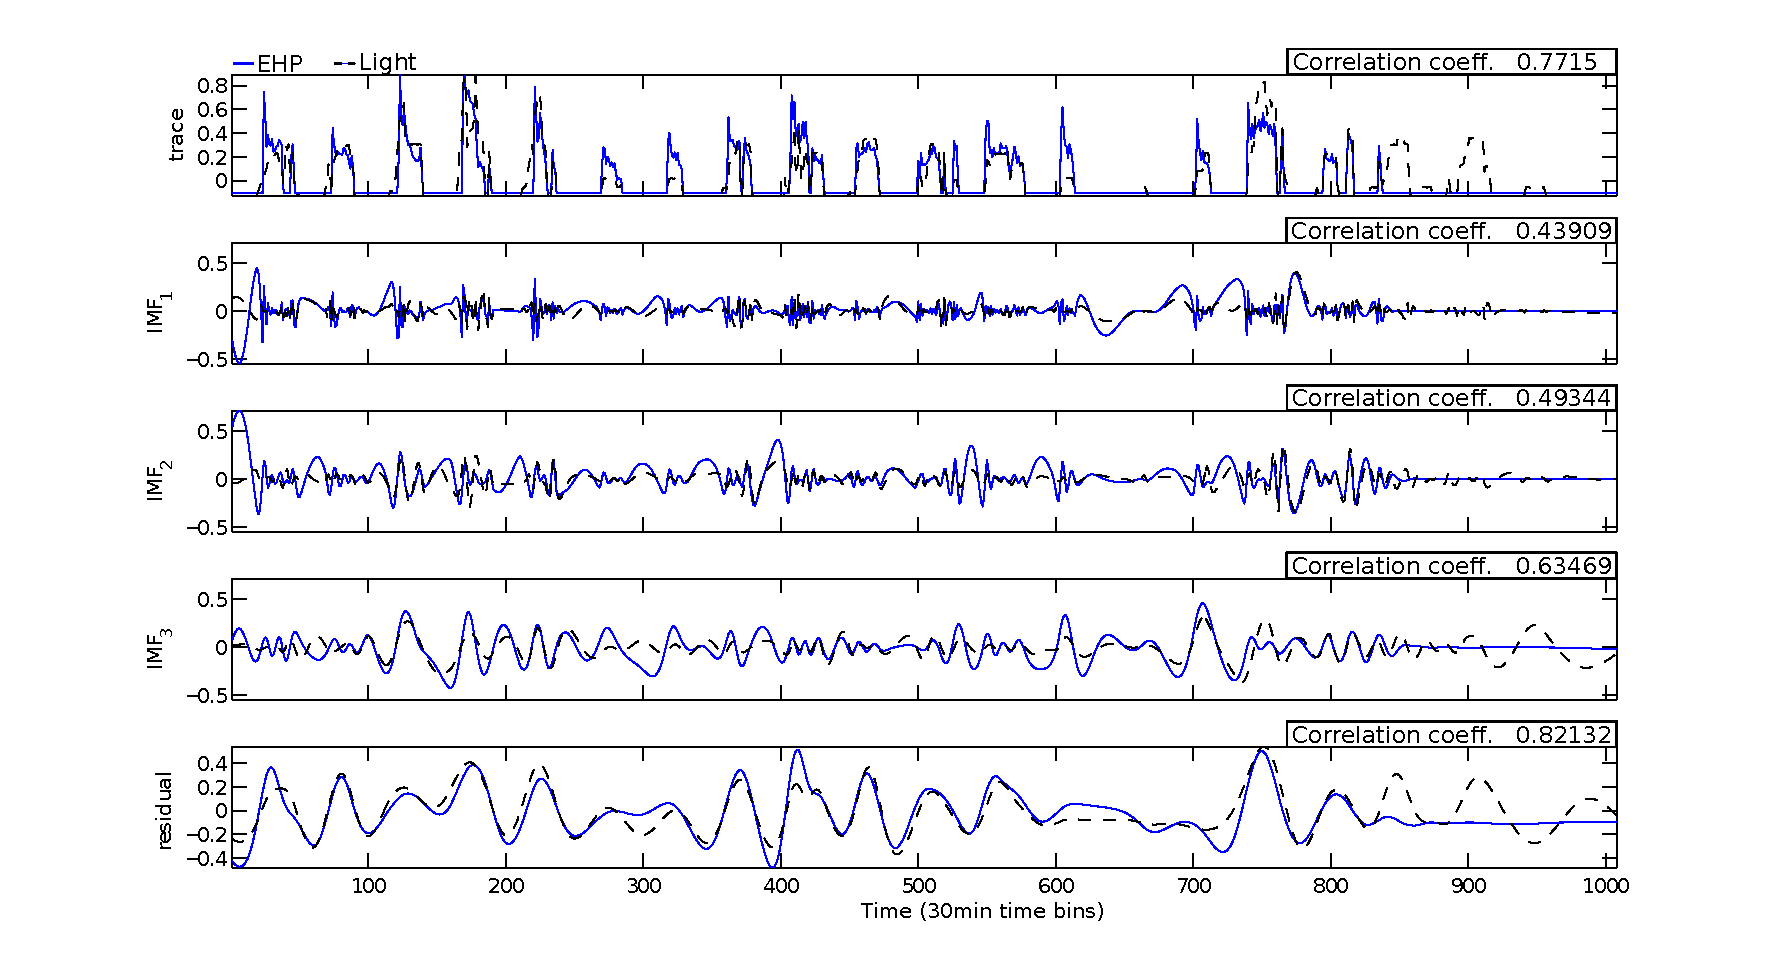
\includegraphics[width=1.2\textwidth]{img/emd_25_26-eps-converted-to}
\vspace{-1cm}
\caption{Decomposition of the EHP and light trace using bivariate EMD. IMFs correlation coefficients highlight the intrinsic relationship of the two traces.}
\label{fig:emd}
\end{figure*}

% The intent of the Green University of Tokyo Project (GUTP) \cite{gutp} is to reduce the university environmental impacts associated to its electric energy consumption.
% The first step of this project was to deploy sensors at the Building No.2 of the Faculty of Engineering 
% Electric power consumption of a 12 floors building containing researchers office and classroom.
% 1215 sensors monitoring different devices...

%received attention in the past \cite{ogawa:lncs2011}.

For this investigation, we focus on a three-week span in the summer of 2011 (from July 4th to July 24th).
The dataset captures regular work days, weekends, and one holiday (July 18th).  This timeframe captures
the typical usage of the equipment, triggered by occupant activity.  For the initial
analysis, we focus on three sensors; two water pumps and a light feed.  The first pump is an 
``electric heat pump'' and is labled as EHP, the second  is a ``gas heat pump''
and labeled as GHP.  The room lighting system serves the same room as the EHP.  The GHP
serve a different room on the same floor.  The expanded portion of our analysis pivots as the EHP
and does a pairwise comparison between it and all other sensors in the building.

% includes one day holiday (July 18th)
% 3 different sensors:
% \begin{itemize}
%  \item Two are measuring the electric power consumption of two devices from the same room; an electric heat 
%  		pump (EHP) and the room lighting system.
%  \item One is measuring the electric power consumption of a gas heat pump (GHP) that is pumping water to cool 
%  		a different room in the same building.
% \end{itemize}

% Later we expand our analysis to include all the sensors in the building.


\section{Problem statement and Initial approach}\label{problem}
% In our analysis, we are focused on finding devices that are correlated in their use over time.  Therefore, the
% main objective is to examine how device traces relate to one another.  The wish to identify
% correlated device-trace patterns at large spatio-temporal scales.

In buildings, metadata is poorly and unsystematically managed within a single system domain.  Moreover, 
with the ever growing number of additional sub-meters, it is important to quickly integrate
sensor data from multiple systems to understand the full state of the building.  It is also important to 
understand how sensors are used in concert.  Anamolies in usage may indicate underlying problems with 
the equipment or inefficient/incorrect usage.  

We begin our analysis by running direct correlation between the traces.
Figure \ref{fig:raw} shows the raw traces for the three devices discussed in 
the previous section (EHP, GHP, light).  All three exhibit a diurnal usage pattern.  On weekends, each
draw less power.  The correlation coefficient for 
 the EHP and light is $0.7715$ and the correlation coefficient for the EHP and GHP is $0.6370$.
Running correlation across them yields high correlation coefficients, mostly
due to their underlying daily usage pattern.

% Usual measures on sensor data like correlation coefficient or granger causality \cite{kim:buildsys2010}
% -- this is not working

\begin{figure}[t!]
\centering
 \subfigure[EHP trace]{\label{fig:raw_ehp}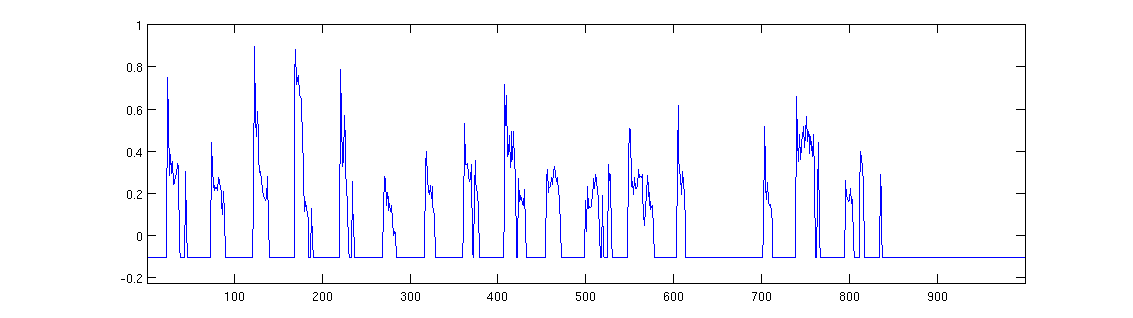
\includegraphics[width=.4\textwidth]{img/25.png}}
 \subfigure[Light trace]{\label{fig:raw_light}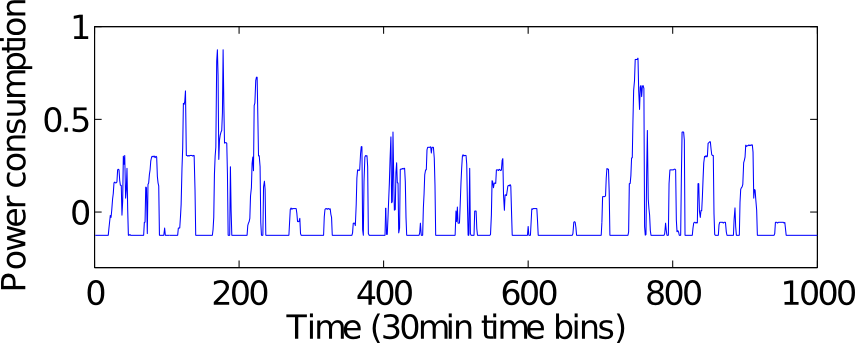
\includegraphics[width=.4\textwidth]{img/26.png}}
 \subfigure[GHP trace]{\label{fig:raw_ghp}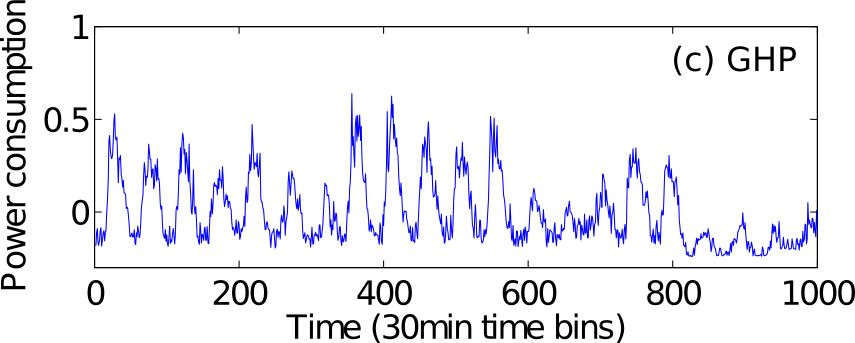
\includegraphics[width=.4\textwidth]{img/41.png}}
 \caption{Traces from three different sensors captured in 2011 from July 4th to July 24th. Data is normalized and aggregated into 30 minutes time bins.}
 \label{fig:raw}
\end{figure}

% For example correlation coefficients for the 3 signals...
% correlation coefficient for the EHP and Light signals: $0.772013$
% correlation coefficient for the EHP and GHP signals: $0.636967$

% These scores suggest that the EHP signal is related to the two other measured signals.

% These results were expected for the EHP and light traces, as the two measured devices operate for the same room 
% and are used simultaneously.  More importantly, they are used to support the occupants of the rooms they are serving.
% We were somewhat surprised by the magnitude of correlation between the pumps, since they serve rooms on
% opposite sides of the building and operate independently.  However, occupancy and weather patterns are similar,
% and the underlying trend is captured by the correlation calculation.
% The difference between the correlation coefficients is small and one might conclude that all three are
% closely related to one another.  That conclusion is not false but misleading.  Correlation on the raw 
% traces is sensitive to the underlying trend shared by the traces.  In order to meaningfully distinguish between
% truly related devices we need to remove the common trends. 

Our initial results were not surprising.  The diurnal pattern dominates the comparison between the sensors.
Weather is the main driver for this behavior and it affects the readings in almost all of the
sensors in our dataset.  Cross-correlation on raw sensor data is insufficient for filtering intrinsically related
behavior.  Upon closer examination of the data we assess the following:

\begin{itemize}
\item The main underlying diurnal trend occurs in almost all the traces.
\item Occupancy and room activities occur at random times during the day and change 
		at a higher frequency than weather patterns.
\item Sensors that serve the same location observe the same activities.  Therefore, their underlying
		measurements should be correlated.
\end{itemize}

In order to uncover these relationships we must remove low-frequency trends in the traces and
compare the readings at high frequencies.

% \begin{table}
% \begin{center}
% \begin{tabular}{|l|l|l|l|l|l|}
% \hline
% × & Raw trace & 1st IMF & 2nd IMF & 3rd IMF & Residual\\ \hline
% EHP, Light & 0.7715 & 0.43909 & 0.49344 & 0.63469 & 0.82132 \\ \hline
% EHP, GHP & 0.6370 & 0.0060274 & 0.063546 & 0.16764 & 0.79378 \\ \hline
% \end{tabular}
% \caption{Correlation coefficients of the analyzed trace and their IMFs uncovered by EMD}
% \label{tab:corr}
% \end{center}
% \end{table}
% \subsection{Simple Scenario}

\begin{figure*}[tb]
\hspace{-2cm}
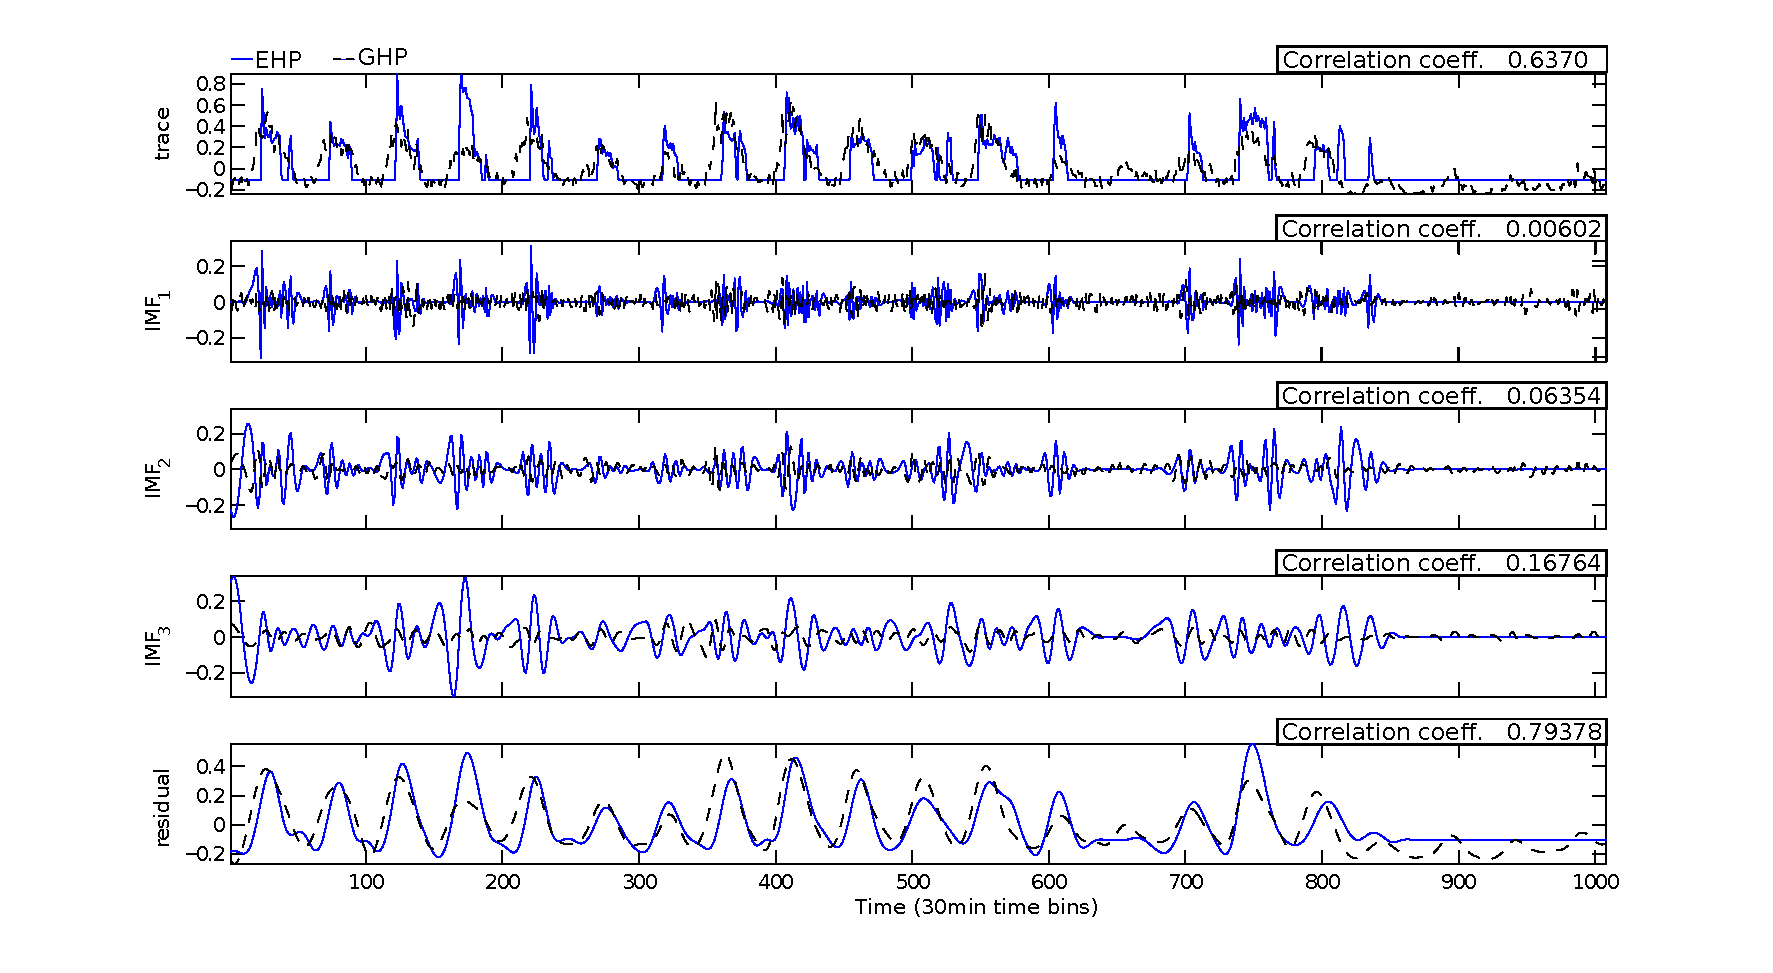
\includegraphics[width=1.2\textwidth]{img/emd_25_41-eps-converted-to}
\vspace{-1cm}
\caption{Decomposition of the EHP and GHP trace using bivariate EMD. IMFs correlation coefficients highlight the intrinsic independence of the two traces.}
\label{fig:emd2}
\end{figure*}

% The small difference between the two computed correlation coefficients is misleading as one could conclude that the three signals are correlated and the corresponding devices are activated by a single action.

% The high correlation coefficients obtained for these three signals result .... weekly pattern....
% small difference = local fluctuation...

% this high score comes from the fact that the two devices are monitoring offices that are weekly used.

% Indeed the weekly pattern of the data trump the correlation coefficients....

% How to inspect only the local fluctuations...?
% we'd like to have an elegant solution (i.e. not specifying the interesting time scale)


\section{Methodology}\label{method}
%Remove the weekly trend of the data to analyze the detailed changes that convey the device behavior at small time scales.

% Our initial approach examined correlation analysis on raw sensor traces.  However, we quickly
% found that correlation is overly sensitive to fluctuations in the data.
Fundamentally, the readings are driven by the same underlying phenomena: 
weather and occupancy.  Weather influences \emph{all} the data similarly.  Occupancy, however, changes
throughout the building and should be used as a differentiating component in the signal
comparisons.  Sensors that share spatio-temporal elements should be correlated after the removal
of the underlying trend driven by the weather.  In order to find unique relationships we needed to remove 
this common trend.

\subsection{Empirical Mode Decomposition}
Empirical Mode Decomposition (EMD) \cite{huang:emd1998} is a new techniques used for de-trending data.
Specifically, EMD detrends non-stationary, non-linear timeseries data.  A trend is defined as 
an intrinsically determined monotonic function within a certain temporal span or a function in which there 
can be at most one extremum within that temporal span.  A non-stationary signal is a signal whose mean and
variance change over time.  EMD is a process, rather than a theoretical tool.

We describe the process as follow:  for a signal \emph{X(t)}, let $m_1$ be the mean of its upper and
lower envelopes as determined from a cubic-spline interpolation of local maxima and minima. The locality 
is determined by an arbitrary parameter.

\begin{enumerate}
\item The first component $h_1$ is computed: $h_1=X(t)-m_1$
\item In the second sifting process, $h_1$ is treated as the data, and $m_{11}$ is the mean of $h_1$'s upper and lower envelopes: $h_{11}=h_1-m_{11}$
\item The procedure is repeated $k$ times, until $h_{1k}$ is a function: $h_{1(k-1)}-m_{1k}=h_{1k}$
\item Then it is designated as $c_1=h_{1k}$, the first functional component from the data, which contains the shortest period component of the signal. We separate it from the rest of the data: $X(t)-c_1 = r_1$, and the procedure is
repeated on $r_j: r_1-c_2 = r_2,\dots,r_{n-1} - c_n = r_n$
\end{enumerate}

The result is a set of functions called intrinsic mode functions (IMF); the number of functions in 
the set depends on the original signal~\cite{emd_process}.  An IMF is any 
function with the same number of extrema and zero crossings, with its envelopes being symmetric with respect to zero.
We run our correlation analysis on the shared IMF outputs between a pairs of signals.  In order to ensure 
that the IMFs corresponding to two distinct signals are on the same time scale, we use 
bivariate EMD \cite{rilling:biemd2007} to decompose two signals at once. The main use of EMD is for removing dominant trends to conduct a meaningful spectral analysis of the data.


\subsection{Results}

We test our hypothesis in this section by using EMD to remove low-frequency trends in the data
and run correlation calculation at overlapping IMF timescales.  We discover that EMD allows us
to find and compare high-frequency instrinsic behavior that is spatially correlated across
sensors.  We begin with a small set of three sensors (EHP, GHP, light) and expand our scope
to include all the sensors in the dataset.



\subsubsection{Initial analysis}
Lets consider the simple example of Section \ref{problem} where we would like to know if the EHP trace is correlated with the two other traces.
Recall that the correlation coefficients of the raw feeds was $0.7715$ and $0.6370$, corresponding to the light 
and GHP, respectively.
As stated in previous section this result is correct but not so meaningful, since most of the traces
display the same diurnal pattern.
Figure \ref{fig:emd} and Figure \ref{fig:emd2} show the EMD decomposition of the three traces.
For each trace, EMD has retrieved three IMFs that highlight the higher frequencies of the traces.

Figure~\ref{fig:emd} shows the normalized raw trace (top) and EMD output IMFs and residual as well as the 
correlation coefficients calculated on the IMFs for the EHP and
light traces.  The correlation coefficients are $0.43909$, $0.49344$ and $0.63469$ corresponding to the IMF1, 
IMF2, and IMF3, respectively.  Notice the high correlation between the high-frequency IMFs.
We know that the light and EHP serve the same room, and their high-frequency IMF correlation corroborates
our prior knowledge.
Figure~\ref{fig:emd2} shows a complementary result, for the EHP and GHP comparison.
The correlation coefficients for the EHP and GHP IMFs suggest that the two may be independent.  In fact, they
\emph{are} indepdent; they serve completely different rooms in the building!

EMD allows us to remove low-frequency trends that add noise to the original analysis.
By comparing IMFs, we see both intrisically correlated and \emph{uncorrelated} behavior.  In the next
section we expand our analysis and show the effectiveness of our methodology. 
% Although promising, these results must be validated across the rest of the
% dataset to confirm their significance.  


\subsubsection{Validation}
To validate the effectiveness of our approach, we analyze the same three-week time span for \emph{all} 674 
sensors deployed in the building.
For each trace $S$ we compute two scores: (1) the correlation coefficient between $S$ and the EHP trace
and (2) the average value of the IMF correlation coefficients.

\begin{figure}[tbh!]
\centering
 \subfloat[Raw traces correlation coefficients]{\label{fig:histo1}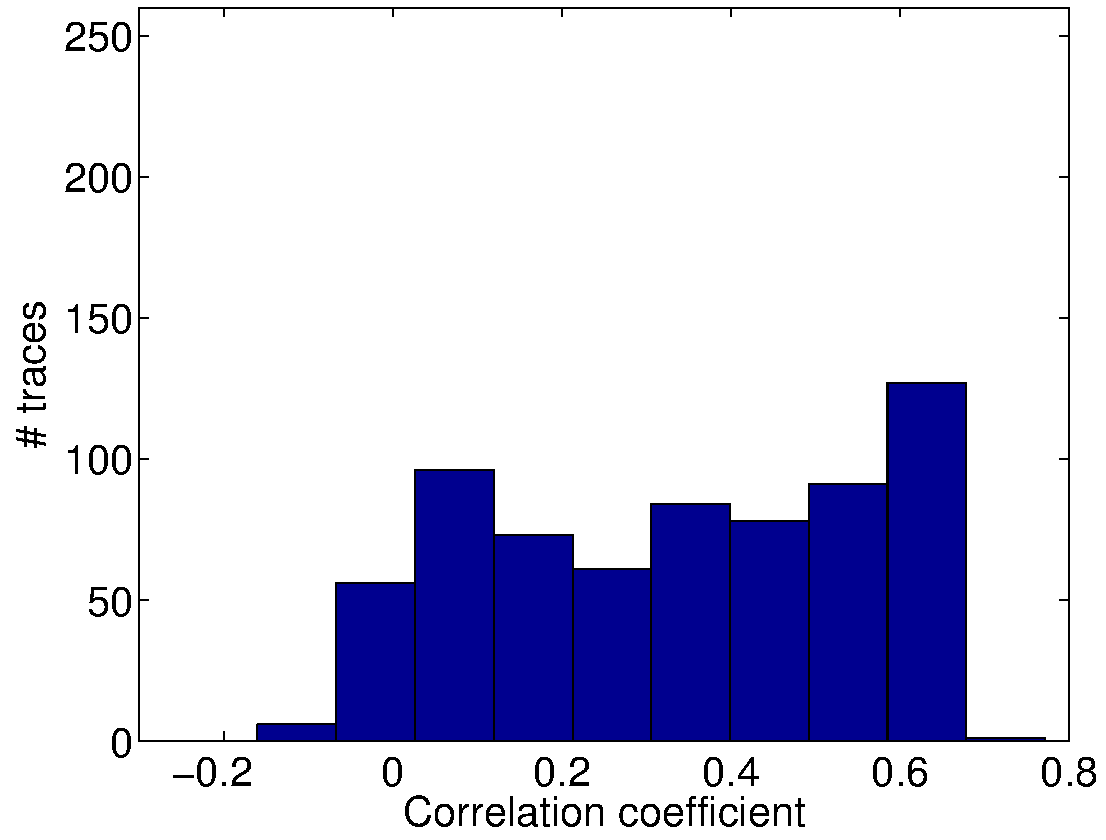
\includegraphics[width=.43\textwidth]{figs/allFloors_week1_week4_corr_abs-eps-converted-to}}
 \subfloat[Average IMFs correlation coefficients]{\label{fig:histo2}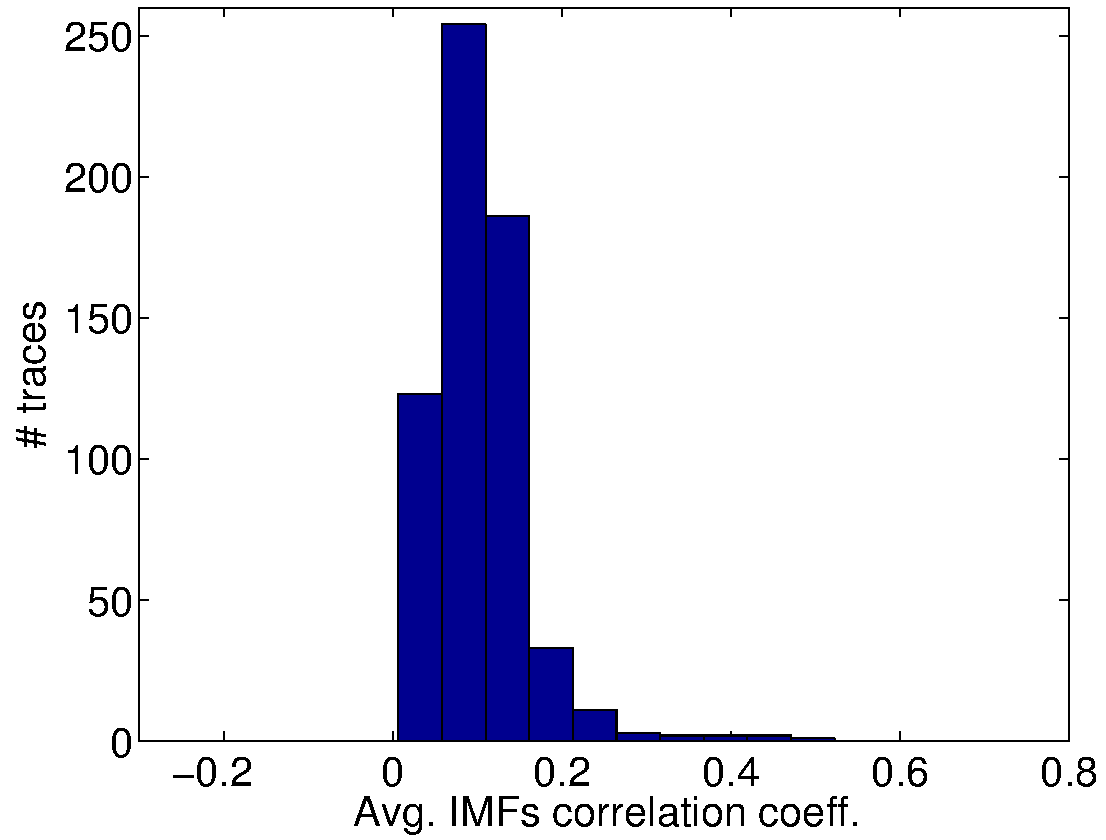
\includegraphics[width=.43\textwidth]{figs/allFloors_week1_week4_emd_abs-eps-converted-to}}
 \caption{Distribution of the correlation coefficients of the raw traces and correlation coefficients average of the corresponding IMFs using 3 weeks of data from 674 sensors.}
\label{fig:histo}
\end{figure}

\begin{figure}
\centering
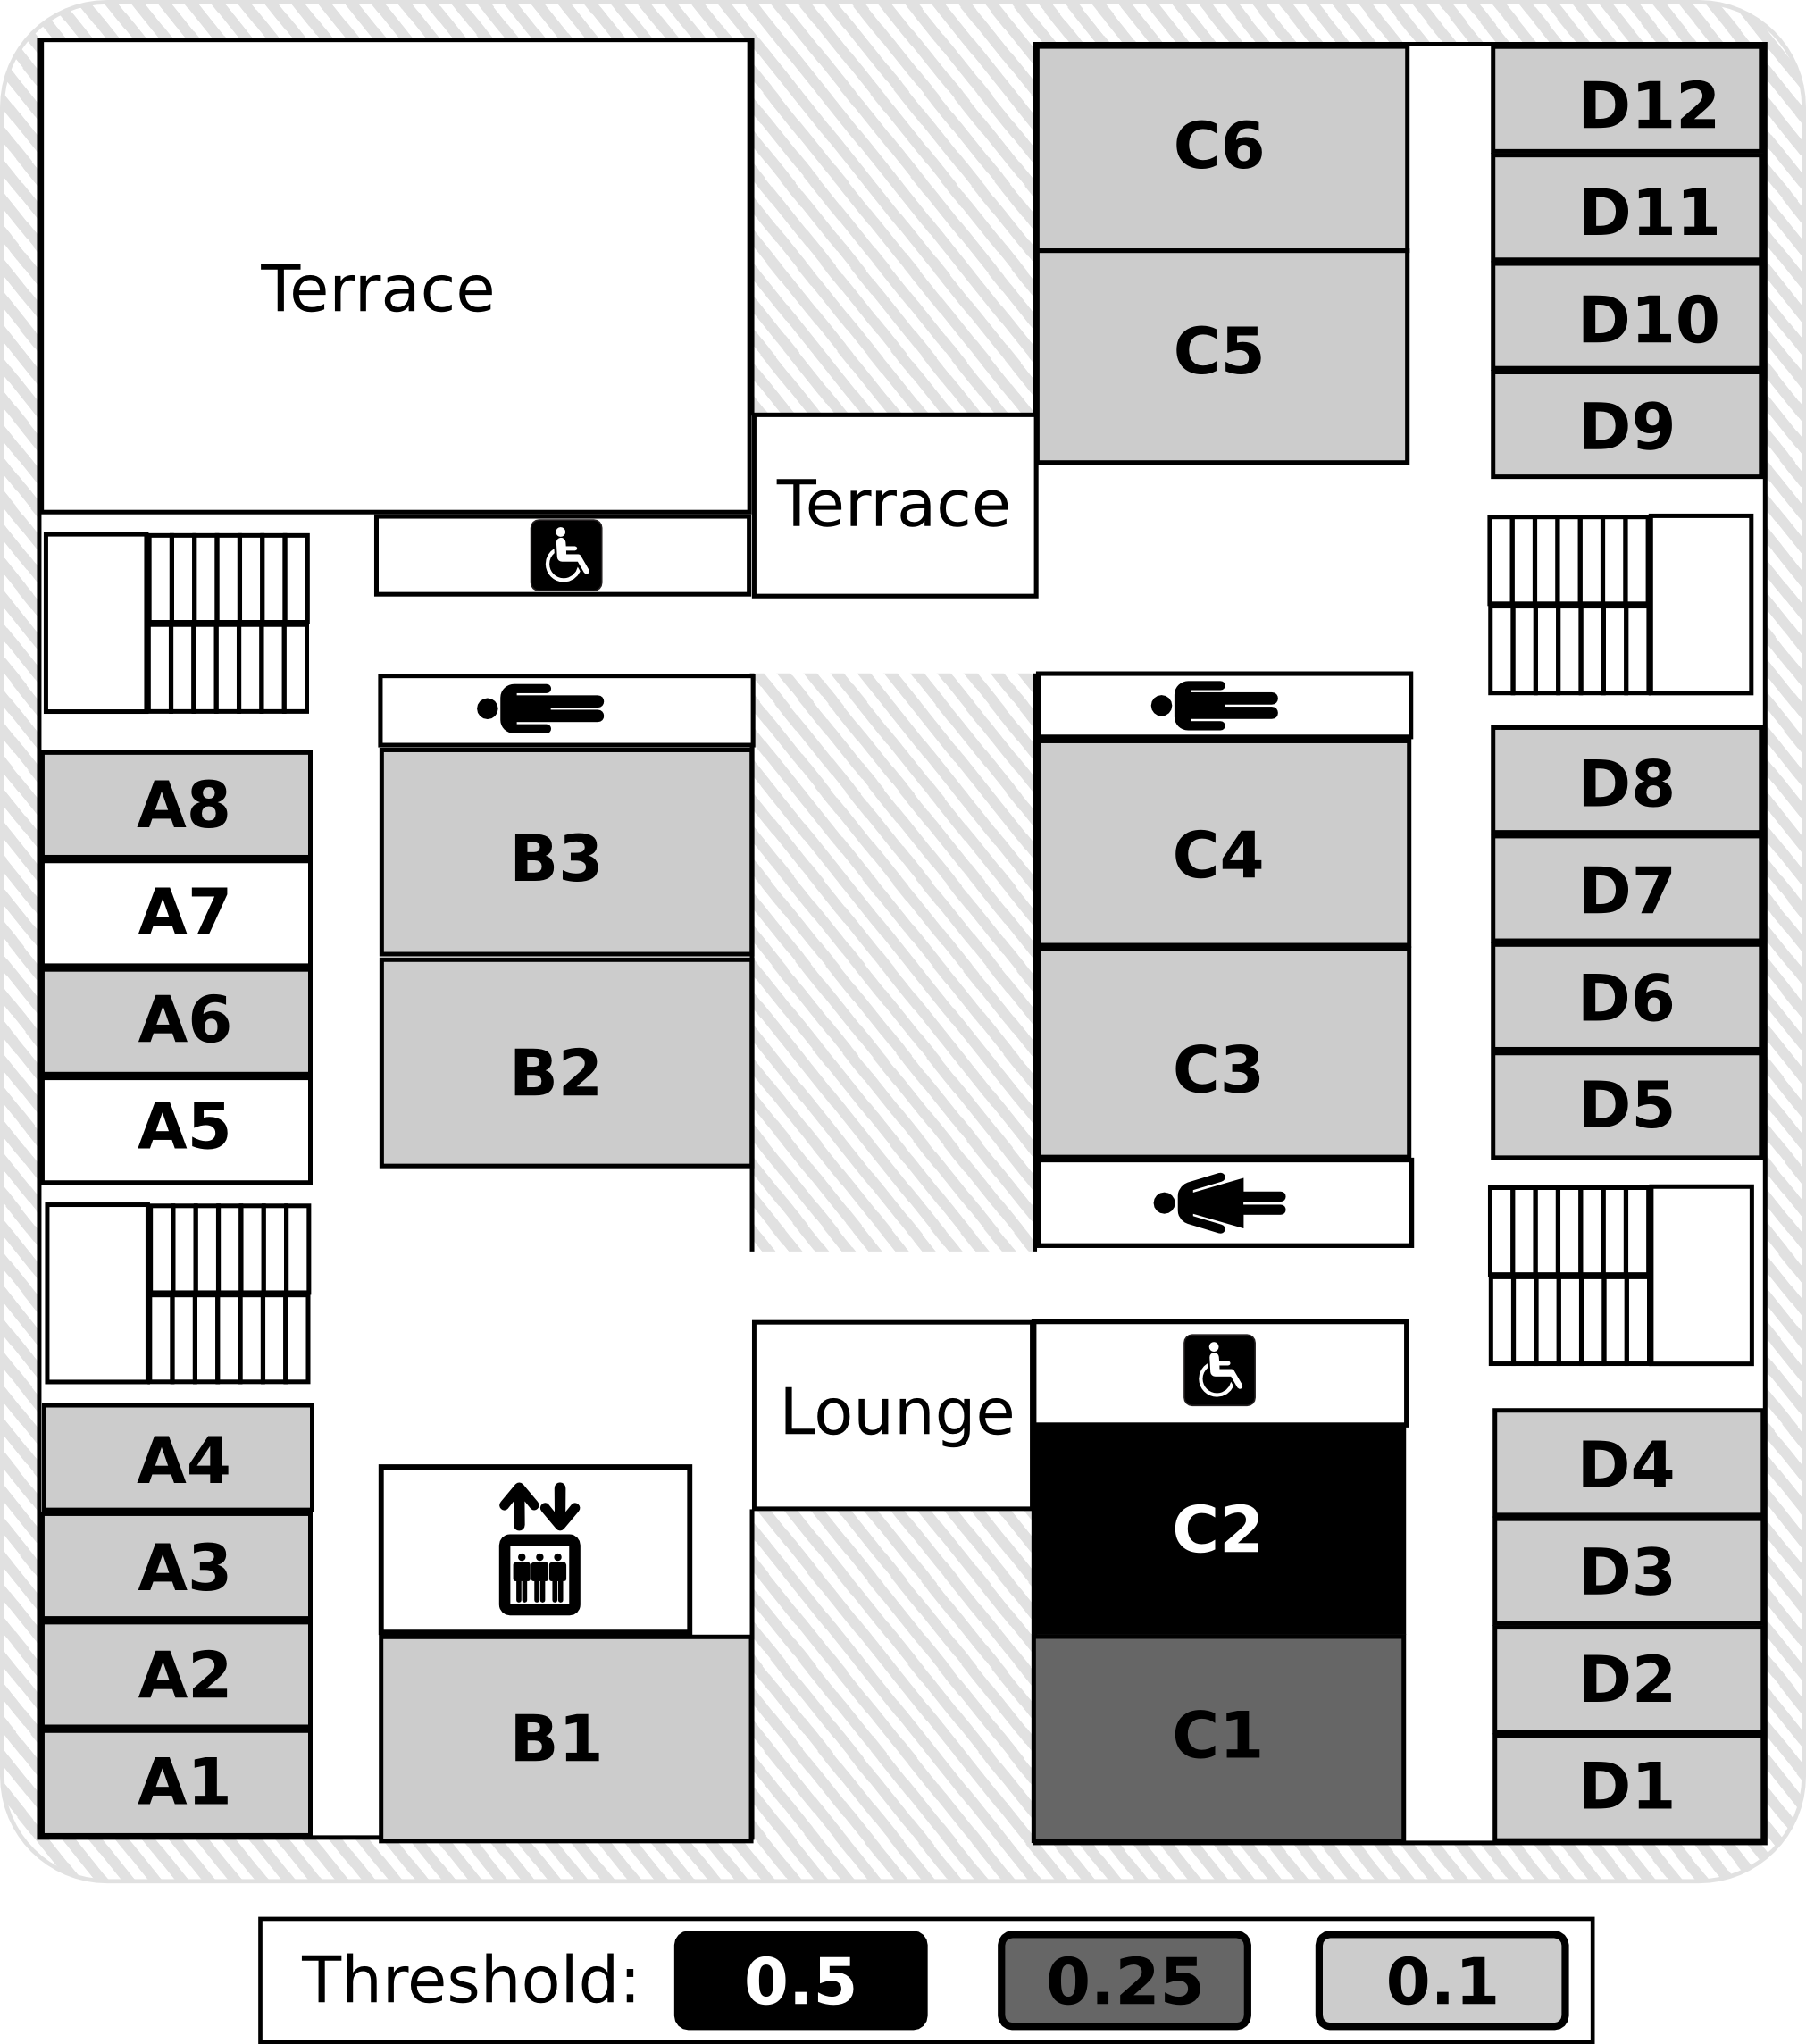
\includegraphics[width=.45\textwidth]{figs/floorMap.png}
\caption{Map of the floor where the analyzed EHP serves (room $C2$). The location of the sensors identified as related by the proposed approach are highlighted, showing a direct relationship between IMF correlation and spatial proximity.}
\label{fig:map}
\end{figure}

Figure \ref{fig:histo1} shows the distribution correlation coefficients.  Notice
that a large fraction of the dataset is correlated with the EHP trace.
\emph{Half} the traces have a correlation coefficient higher than $0.36$.  As expected, the underlying
trend is shared by a large number of device.
Although the highest score (i.e. $0.7715$) corresponds to the light in the same room that the EHP serves,
there are 118 pumps, serving all areas of the building, with a correlation higher than $0.6$.
Using only these results, it is not clear where the threshold should be set.  The distribution is close to 
uniform, making it difficult to 
know of how well your threshold discriminates against unrelated traces.
% Moreover, the distribution of the traces is almost uniform, thus, discriminating correlated traces is a laborious task.

Figure \ref{fig:histo2} shows the distribution of the average correlation value for the IMFs of
each trace and the EHP.  The number of traces correlated in the high frequency IMFs is significantly smaller
than the previous results. It's clear from the distribution that only a small set of devices are
\emph{intrinsically correlated} with the EHP.  In fact, \emph{only 10 traces out of 674} yielded a score higher than 
$0.25$. This allows us to easily rank traces by correlation.

Upon closer inspection of the 10 most correlated IMF traces, we find that there is a spatial relationship
between the EHP and the ten devices.  In fact, there is a direct relationship between score and distance from
the areas served by the EHP.  Figure~\ref{fig:map} shows a map of the floor that contains the rooms served by this
EHP.  The EHP directly serves room $C2$.  We introduce a correlation threshold to cluster correlated traces by score.
We highlight rooms by the threshold setting on the IMF correlation score.
When we set the threshold at $0.5$ we see that the sensors that have a correlation higher fall within room $C2$ --
the room served directly by the EHP.  As we relax the threshold, lowering it to $0.25$ and $0.1$ we see radial expansion from $C2$.  The trace with the highest score, $0.522$, is the trace corresponding to the lighting system \emph{in
the same room}.
The two highest scores for this floor (i.e. $0.316$ and $0.279$) are the light and EHP traces from next door, room $C1$.
Lower values correspond to sensors measuring activities in other rooms that have no specific relationship to the analyzed trace.  The results show a direct relationship between IMF correlation and spatial proximity and \emph{supports our initial
hypothesis}.


% Interestingly, the IMFs correlation coefficients reveal the spatial correlation of the sensors.
% Figure \ref{fig:map} is the map floor where the EHP trace is measured.
% Specifically, the EHP reports heating activity in the room $C2$.
% in the simple scenario the GHP is located in the room A5.



\subsection{Limitations}
EMD is useful for finding underlying behavioral relationships between traces of sensor data.  However,
when we set the timescales smaller than a day, the results were not as strong.
The trace has to be long enough to capture the trend.  For this data set, the underlying
trend is daily, therefore it requires there to be a significant number of samples over many days.
%  to
% for this method to be effective.
Although this was a limitation for this dataset, it really depends on the underlying phenomenon that
the sensors are measuring.  Its underlying trend is ultimately what EMD will be able to separate
from the intrinsic modes of the underlying signal.

\subsection{Discussion}
EMD allows us to effectively identify fundamental relationships between sensor traces.
% Using EMD to find fundamental relationships between sensor traces effectively identifies intrinsically
% related behavioral relationships.
% was quite promising for building
% up models of correlated usage.  
We believe that identifying meaningful usage-correlation patterns can help reduce oversights
by the occupants and faults that lead to energy waste.  A direct application of this is the identification
of simultaneous heating and cooling~\cite{simheatcool}.  Simultaneous heating and cooling is when heating
and cooling system either compete with one another or compete with the incoming air from outside and is
a cause for major energy waste in building~\cite{simheatcool}.  The longer it goes undetected,
the more waste there is.  However, it is very difficult to identify since the occupants do not notice
changes in temperature.  Our analysis can be used to build a correlation model between the outside
heating cooling temperature, the cooling coil temperature, and the outside air vent position.  If their behavior
is not correlated as expect, an alarm should be raised.

We can also apply it to other usage scenarios.  In our traces, for example, we found an instance where the pump
was on, but the lights were off.  The two are typically correlated, however, in this case they were not.
The air conditioning was pumping cool air into a room without occupants.
With our approach this could have been identified and corrected.  In future work, we intend to
package our solution to serve these kinds of applications.

% EMD works perfectly although the weekly pattern of the data is altered the last analyzed week.

% EMD inherently finds the interesting time scales.

% number of zero crossing = mean frequency/time scale:
%   TODO give the time scale for each IMF.


\section{Conclusion}
% what is our problem

% what we did

% contributions and main results

% future work


This paper set out to examine the underlying relationship between sensor traces to find interesting correlations
in use.  We used data from a large deployment of sensors in a building and found that direct correlation analysis on the raw
traces was not discriminatory enough to find interesting relationships.  Upon closer inspection, we noticed that
the underlying trend was dominating the correlation calculation.  In order to extract meaningful behavior this trend has
to be removed.  We concluded that empirical mode decomposition is a helpful analytical tool for de-trending 
non-linear, non-stationary data; inherent attributes contained by our traces.

We re-ran our analysis on the same traces, except we correlated the IMF outputs of the EMD operation on each of the traces and found that the pump was closely related to the lights in the same room served by the pump and
uncorrelated with a pump on the same floor serving a different room.  In order to corroborate the applicability
of our approach, we compared the pump trace with \emph{all} 674 sensor traces and found a strong correlation
between the relative spatial position of the sensors and their IMF correlations.  The most correlated IMFs were 
serving the same
area in the building.  As we relax the admittance criteria we find that the spatial correlation expands radially from
the main location served by the reference trace.

We plan to examine the use of this method in applications that help discovery changes in underlying relationships over time
in order to identify opportunities for savings in buildings.  We will use it to build inter-device correlation models
and use these models to establish ``normal'', ``abnormal'' usage patterns.  We hope to take it a step further and include a
supervised learning approach to distinguish between ``efficient'' and ``inefficient'' usage patterns as well.









\section{Functional Verification through Classification and Experimentation}
\section{Value-Based Verification Through Physical-Model Checking}
\section{Related Work}
\section{Summary}



% \chapter{Timeseries Data Processing}

% \section{Collection and Storage of Phyiscal Data}

% \section{Data Processing: The File System Metaphore}







\chapter{Building Metadata}
\subsection{Building Entities}
\subsection{Entity Relationships}

\section{Constructing Multiple Views}
\subsection{Capturing System Relationships}
\subsection{Capturing Spatial Relationships}
\subsection{Capturing Functional Relationships}

\section{Queries in the Built Environment}

\section{Related Work}

\section{Remaining Challenges}



\chapter{Architectural Evaluation}


\section{Visualization and Analysis of Streaming Data}

\section{Energy Audition with Mobile Phones}

\subsection{Introduction}
The United States leads the world in per-capita energy consumption.
Our electricity use has consistently increased over the last 40 years~\cite{oecd2011} and other parts of the world are rising all 
too rapidly.  With the specter of climate change and the increasing cost of energy, we must explore new
ways for individuals to gain visibility and insight into their energy consumption in order to optimize and reduce it. 
With the increasing penetration of embedded sensors in the environment and
the continued rise in smartphone adoption, we see an opportunity for smartphones to bridge the physical world
to our computational infrastructure and provide an `energy lens' on the physical world.  

We use mobile phones to construct an entity-relationship 
graph of the physical world and combine it with streaming sensor data in order to perform detailed energy-attribution.
We limit the scope of the world to a single building domain.  We have designed and implemented a real-time, mobile energy auditing
application, called the `Energy Lens', that allows us to collect information about 
things throughout the building and how they are related to each other.  For example, computer X is inside 
room Y and connected to meter Z.  Then, we use these relationships to guide our data look-up and analytical
calculations.  For example, the load curve of room Y consists of the sum of all the power traces for loads
inside room Y.  We use the mobile smartphone as the main input tool.  Our work examines \emph{three main challenges} in setting up and 
deploying a real, whole-building infrastructure to support real-time, 
fined grained energy analytics.  

The first challenge is related to tracking and mobility.
The use of mobile phones presents classical, fundamental challenges related to mobility.  Typically, mobility
refers to the phone, as the person carrying it moves from place to place.  However, in the energy-attribution
context, we are also referring to the movement of energy-consuming objects.  Tracking their relationships to spaces 
and people is as important as tracking people.  We describe how we deal with \emph{both moving people and 
moving objects} and show that these historically difficult problems can be addressed relatively easily, if the proper infrastructure is 
in place.  %We provide evidence that the approach is simple, incrementally deployable, and scalable.

The second challenge is about capturing the inter-relationship semantics and having these inform our  analytics.
We adopt the general notion of physical tags that identify objects in the world.  Our system uses \emph{QR codes} to tag things and locations 
in the physical world.  However, \emph{any tag that provides a unqiue identifier for an object could serve the same purpose}.
Once tagged, there are three types of interactions -- 
registration, linking, and scanning -- which establish important relationships.  Registration is the act of creating a virtual object 
to represent a physical one.  Linking captures the relationship between pairs of objects.  Scanning is the act of performing an item-lookup.
Each of these interactions requires a set of swiping gestures.  Linking requires two tag swipes while the other two actions
require a single tag swipe.  Internally, we maintain a \emph{entity-relationship graph (ERG)} of things, people, and locations, that gets
updated through these sets of gestures.

The third challenge is about indoor network connectivity and access.
In order to connect these components, we rely on having `ubiquitous' network connectivity.  However, in practice, network
\emph{availability} is intermittent and our system must deal with the challenges of intermittency.  We discuss how caching
and logging are used to address these challenges.  Moreover, when connectivity is re-established, we must deal with
applying updates to the ERG, as captured by the phone while disconnected.  
% Conflicts can also occur during an update.  For example, the two updates may disagree about which items are attached
% to which meters.  We implement a very simple conflict resolution scheme, described in section~\ref{sec:conflicts}.
% Finally, certain physical-state transitions are represented as a set of updates to the ERG that must be applied 
% atomically.  We implement transactions in the log-replay and transaction manager.
% Our `Energy Lens' system is deployed in a building on our campus.  We discuss
% its architecture and our design choices.  
  
% We also discuss novel strategies for tracking moving people/things and describe how we implement these in our system.  In summary, our work
% makes the following contributions:

% \begin{itemize}
% \item We design and implement a system that captures and combines physical entities, their inter-relationships, and real-time sensor data 
% 		in buildings.% using mobile phones, qr code, and a cloud-based infrastructure.
% \item We observe that certain combinations of swipes give us useful information to set the location of people and things over time.
% 		We codify this observation in our \emph{context-tracker} and use it to maintain consistency between the entity-relationship graph and the 
% 		state of the physical world.  To the best of our knowledge, this is radically different from the approaches in standard 
% 		localization techniques.  However, we argue that it can be used to \emph{enhance} their accuracy and overall performance.
% \item We implement a prefetching algorithm to obtain context-dependent information to both improve performance and
% 		enable disconnected operation.  We also design and implement a log-replay and transaction manager over our data management layer.  We describe how different conflict-resolution policies can be implemented and our rationale for the policies we chose.
% \end{itemize}

% \vspace{0.08in}

% In the next sections we go through a motivating scenario.  We then discuss some related work, followed 
% by the system architecture, evaluation, and future directions.

\section{Motivating scenario}
\label{sec:vision}
% Several things to mention:

% \begin{itemize}
% \item physical data services
% \item energy analytics
% \item we need to know where things are, people are, how they're inter-related
% \item integration of all building energy feeds into one system
% \end{itemize}

Imagine having the ability to walk through a building and see live, detailed energy-attribution data as
you point your phone at various things and locations.  As you enter your work office building, you scan its tag and see
the live breakdown of energy consumption traces, including HVAC, lighting, and plug-loads.  You continue
your walk through the building as you head to your office.  When you step out of the elevator on your floor
you scan the tag for the floor and observe similar figures, only this time they are in relation to that floor
alone.  Since there are several meeting rooms on that floor, you are curious how much is consumed by 
occupants versus visitors.  You choose to view the total load curve co-plotted with the occupant
load curve, specifically for that floor.  You see that approximately half the total energy is consumed
by visitors during the day.  You're curious what portion of those figures can be attributed to you, so you select the 
personalized attribution option and you see your personal load curve plotted
with the total load curve, as well as accompanying statistics, such as the percent of total over time.
As you quickly examine the data on your phone, you see that you consumed energy during hours that you were not
there.  You choose to see a more detailed breakdown.  You enter your office, scan the various items and see that
your computer did not shut down properly and your light switch was set to manual.  You immediately 
correct these.

Being able to interact with your environment and get a complete energy break-down can provide a useful tool
for tracing and correcting rampant energy consumption.  In buildings, having the occupants actively participate
allows for localized, personal solutions to efficiency management and is crucial to scaling to large buildings.
However, providing this detailed level of attribution is challenging.  There's lots of data coming from various systems 
in the building, and integrating them in real time is difficult.  Furthermore, attribution is non-trivial.  At the
centralized systems level, some systems service multiple locations and it is non-trivial to determine the exact
break-down by location.  At the plug-load level, some plug loads move from place to place throughout the building.
For example, we must be able to answer: How much of the total consumed on this floor went to charging laptops?  How
many of those charging laptops belonged to registered occupants of this floor versus visitors?

Answering the query is relatively trivial once if the information is available, however, collecting the information
is non-trivial.  Historically, it has been difficult to collect plug-load information.
Various studies have used wireless power meters to accomplish just this~\cite{stephscale, lanz, aceee}.
All previous work collected the data and performed post-processing to analyze it.  We want to take the next
natural set of steps: perform processing in real-time and present the occupants with live information.  
% We also
% aim to integrate it with other live data streams, like those coming from the building management system (BMS).
There are several systems challenges that must be overcome in order to achieve this vision.  We need to 
place live metering on plug loads.  We need to integrate data from the BMS with plug load and other
meter data.  We need to be able to approximate the attribution algorithms and tailor them for real-time processing.
Most importantly, we need to deal with the systems challenges for tracking which things belong to whom, where people
and things are over time, how to deal with the mobile phone as the main interactive modality, and how to do this at the scale of 
hundred to thousands of users and live meter data.  We argue that \emph{without addressing these systems issues, this
vision cannot be achieved}.  In our work, we start by deploying a network of wireless power meters and use the mobile
phone to re-create a model of people, things, and locations in the building.  We also use it to assist in tracking of 
people and things over time.


\section{Related work}

%\begin{itemize}
% \item dashboard
% \item andrew's lightin control work
% \item Kamin's hvac control work
% \item BEMs
% \item sMAP stuff
%\item Buildsys 2010 work~\cite{hbci}
%\item distributed consistency management: COPS
%\item mobility: tracking things with RFID~\cite{rfid_gonz2006}
%\item mobility: tracking of people, wifi indoor localization
%\item entity-relationship graphs
%\item homeOS [microsoft]
%\item HP Cooltown~\cite{cooltown}
%\end{itemize}
Our work touches on several areas from smart home research to logistics.  In the building space, there has been
some interest in building various kinds of energy-related visual and control applications.
This work focuses on the object definition, tracking, and management component of the architecture proposed by 
Hsu et al.~\cite{hbci}.  Their work stratefied the set of challenges that one could potentially face if the application 
were deployed at scale.  Our
work, in constrast, bases its design rationale on a \emph{real deployment} that is taking place at scale in a building 
on our campus.  We focus on solving fundamental systems challenges in dealing with intermittent connectivity
and conflict resolution in tracking people and things over time.  We also focus on leveraging gestures to minimize
the cost of interaction for users, while maximizing the information we can attain about the state of the world.

% Tracking people/indoor localization
An important aspect of the Energy Lens is determining when people and things have moved.  This requires some form 
of indoor localization.  There's a large body of literature in the area of indoor localization with mobile phones ranging from 
using wifi~\cite{radar}, to sonar~\cite{cricket}, to ambient noise~\cite{abs}, and a combination of sensors on the 
phone~\cite{surroundsense, darwinphone}.  Dita~\cite{dita} uses acoustic localization of mobile phones and also uses the infrastructure 
to determine gestures in free-space that are classified into pre-defined control actions.  Each of these require relatively complex 
software and/or infrastrure.  
We take a radically different, simple approach.  We use cheap, easy to re/produce tags (QR codes), place them on things in the 
environment over incrementally and use the natural \emph{swiping gesture} that users make, when interacting with the Energy Lens 
application, to track when they have moved or when the objects around them have moved.  The working principal is to attain as much 
information from their gesture to determine when something/one has moved.  We discuss our heuristics in section~\ref{sec:swipes}.

% context-aware apps
ACE~\cite{ACE} uses various sensors on the phone to infer a user's context.  The context domain consists of a set of user activities
and semantic locations.  For example, if ACE can distinguish between {\tt Running, Driving, AtHome, or InOffice}.  ACE also infers 
the one from the others, so if the user is {\tt AtHome} then they are not {\tt InOffice}.  Energy Lens uses inference to determine
when a person or thing has moved.  Certain swipe combinations give us information about whether they moved and where they moved to or
whether an item moved and where it moved to.  The main difference is that we only infer context when a user is actively swiping, rather
than a continuous approach.  Pretching is a fundamental technique used in many domains.  However, the cost of a prefetch for mobile
application outways the benefits if the prefetched data is not useful.  Informed mobile pretching~\cite{IMP} uses cost-benefit analysis 
to determine when to prefetch content for the user.  In the Energy Lens context, we prefetch data based on their location swipes.
We also rely on pretching to anticipate loss of connectivity, not just to improve preformance.

% Tracking things
Logistic systems focus on the tracking of objects as the move through distribution sites to warehouses, stores, shelves,
and purchase.  Items are tracked through bar code or RFID readers.  However, the workload is very structured and well
defined.  The authors of~\cite{rfid_gonz2006} describe this structure and leverage it to minimize storage
requirements and optimize query-processing performance.  Energy Lens uses the QR codes as the tag and the phone as an active
reader.  As objects move, users scan those items to their new location.  However, objects may belong to one or
many people, they can be metered by multiple meters a day, and their history in the system
is on-going.  In contrast, a typical logistics workload has a start (distribution site) and end point (leaving the store
after a sale).  In our workload, relationship semantics are important; we need to know whether the meter is \emph{bound-to}
rather than simple \emph{attached-to} an item.  We discuss the difference later in the paper.
% In addition to traditional logistics-style queries -- \emph{What is the average time that it took coffee-makers to move from the 
% warehouse to the shelf and finally to the checkout counter in January of 2004?} -- energy-analytics requires queries to group
% partial traces from meter data by tracking what meters the item attached to over the specified time-frame.
% The Energy Lens system collects and manages this kind of information to enable such queries.
Furthermore, we take advatange of natural gestures the user makes with the phone while scanning QR codes to extract
information about the current location of the user or things.

% Tagging items, virtual services
The key idea in the HP Cooltown~\cite{bridgingphysical,cooltown} work is to web-enable `things' in the world, grouped-by
`place', and accessed by `people' via a standardized acquisition protocol (HTTP) and format (HTML, XML).  
Cooltown creates a web presence for things in the world either directly (embedded web server) or indirectly 
(URL-lookup tag) as a web page page that display the services it provides.  Many of the core concepts in Cooltown 
also show up in Energy Lens.  The main overlap is the use of tags in the world that contain a reference to a virtual 
resource, accessible via HTTP through
a network connection.  Cooltown, however, explicitly chooses not maintain a centralized relationship
graph, it leverages the decentralized, linking structure of the web to group associated web pages together.
Furthermore, things are assumed to not move.  People are the main mobile entities.  The kind of applications
we wish to support must track where things are and their specific inter-relationships.  We imposed a richer set of 
semantics on our, centrally maintained, relationship graph and use it to provide detailed energy information.


\section{System architecture}
The Energy Lens application aims to approximate the vision described in section~\ref{sec:vision}.  For our initial
attempt, we tagged items in a building with QR codes and allowed users to 1) register new items and tag
them with QR codes they can print from the Energy Lens site, 2) tell us which meters are attached to which items,
3) scan individual item to view their load curve over a 24-hour period.

The architecture consists of three layers: the sensing and tag layer, the data management and processing layer, and the application
layer.  In this section we discuss each layer and their most important components.  Each layer in the architecture
is carefully design to work on a real deployment with live users.  In deploying the application in a real building, we ran
into various issues that informed our design.  For example, \emph{QR code reading times vary substantially across phones
and lighting conditions}.  You must design for the least-common demoninator in terms of camera quality and lighting.

Another aspect to consider is network connectivity.  Within our building deployment, connectivity is ubiquitous, connectivity
can still be intermittent.  Connectivity may be lost for several reasons, including disassociation from an access point due
to idleness, dead spots in the building where connectivity to both wifi and 3G/4G are unavailable, multipath-induced
destructive interference, and various other reason.  Dealing with these throughout the data collection and update phase is
especially troublesome.  We discuss various mechanisms and algorithms for dealing with disconnected operation.

\subsection{Sensing and tag layer}
We deployed 20 ACme power meters~\cite{acme} on a single floor of a building on campus.  The data was made available through
sMAP~\cite{smap} and forwarded through our processing and data management layer, StreamFS~\cite{streamfs}.  We distributed
the ACmes throughout a single floor in our building and registered various plug loads as being measured by them.  We also tagged
hundreds of items and locations throughout the entire building.  In addition to tagging the 20 ACmes and the plug-loads they are
attached to, we also tagged 351 unmetered items and 139 rooms with QR codes.

\subsubsection{QR code design}
\label{sec:qrc}
QR codes must be designed to minimize scanning time.  As we iterated through various designs we noticed that dim lighting conditions
and poor cameras on certain phones caused the scan time to increase significantly.  The variance in scan time was high and
very frustrating to deal with.  Without correcting this, occupants will not engage with the application, behavior similar to attaining
user engagement on the web.

% \subsubsection{Usability (Strong dependence of occupants/users)}
% \begin{enumerate}
% \item Minimal number of swipes (protocol description)
% \item minimal amount of textual input (protocol description)
% \item piggy-backed movement classification of people and objects. (protocol description)
% \item QR code engineering to minimize swipe time (swipe times)*
% \end{enumerate}



% A QR code is a two-dimensional barcode that may encode almost 3000 bytes of data.  QR code generators
% can be found on the internet~\cite{qrcgen1, qrcgen2}.  
% Extending the approach in \cite{hbci}, in
% our
% architecture the QR code contains a meaningful {\tt URL} that a
% generic browser can access to provid ea human readable document with complete
% information about the item or space, as well as the additional
% information to bootstrap the smartphone to optimized access, such as
% native apps for interacting with the item or space.  Secondly, the 
% {\tt URL}  must be easily transformed into one that will yield a
% programmatic document, such as a JSON object, that apps can
% manipulate.  And finally, the representation of the URL itself can be
% parsed and utilized locally by native apps, typically by lookup, to
% permit rapid interaction with the item or space.

% \begin{figure}[htb!]
% \begin{center}
% 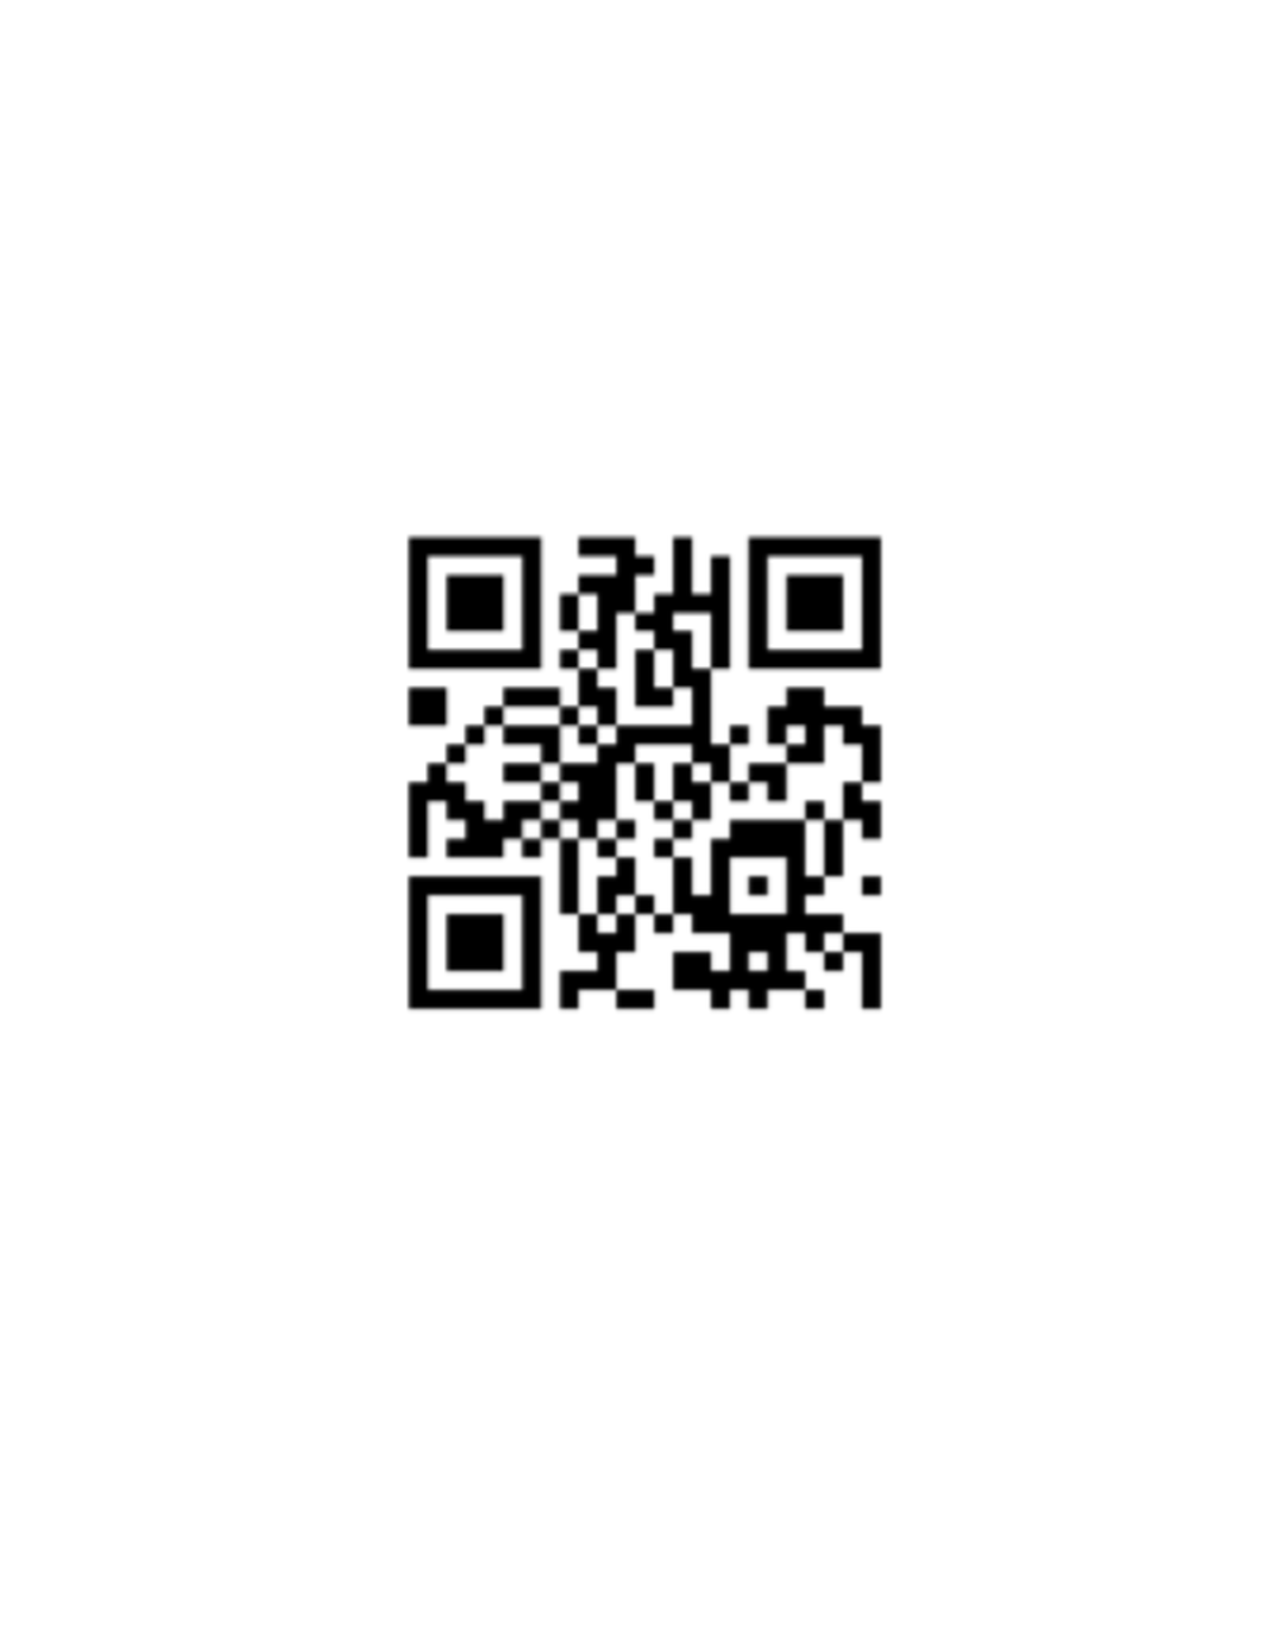
\includegraphics[scale=0.3]{figs/qrcex}
% \caption{This is an example QR code from our deployment. This label resolves to {\tt http://tinyurl.com/6235eyw}.
% QR codes like these are used as tags physical objects and spaces/locations.}
% \label{fig:qrcex}
% \end{center}
% \end{figure}

Figure~\ref{fig:qrcexcomp} shows an example QR code used in our deployment.  Tags like these are placed on physical
objects and spaces throughout the building to link between the physical world and our virtual representation of it.
QR codes are cheap to produce.  Any printer and some tape can be used to tag an item.  This is important for scalability.
With the number of physical objects and places (floors, rooms) in a typical building, {\bf we must rely on the occupants
to scale our deployment}. Because QR codes are easy to produce, we can provide occupants with a webpage that
that produces them.  They print them out, place them on items or
places they want to interact with, register them, and provide useful
information about them.

Generating the right kind of QR code is important.  It is trivial to
encode information onto them, but it is
not trivial to design them so that they encode just enough information to be useful.  If 
too much information is encode the camera takes a long time to scan them, especially under poor lighting
conditions.  This can easily frustrate and drive away users, who are critical for scalability.
We also want to design them for the lowest common denominator in terms of camera quality.  Older
phones with cheap cameras should also be able to scan the tags quickly.  We ran some experiments to show
how complex QR codes differ from the one we design and discuss these results in Section~\ref{sec:qrcexcomp}.

\subsubsection{QR code swipe times}
\begin{figure*}[htb!]
\begin{center}
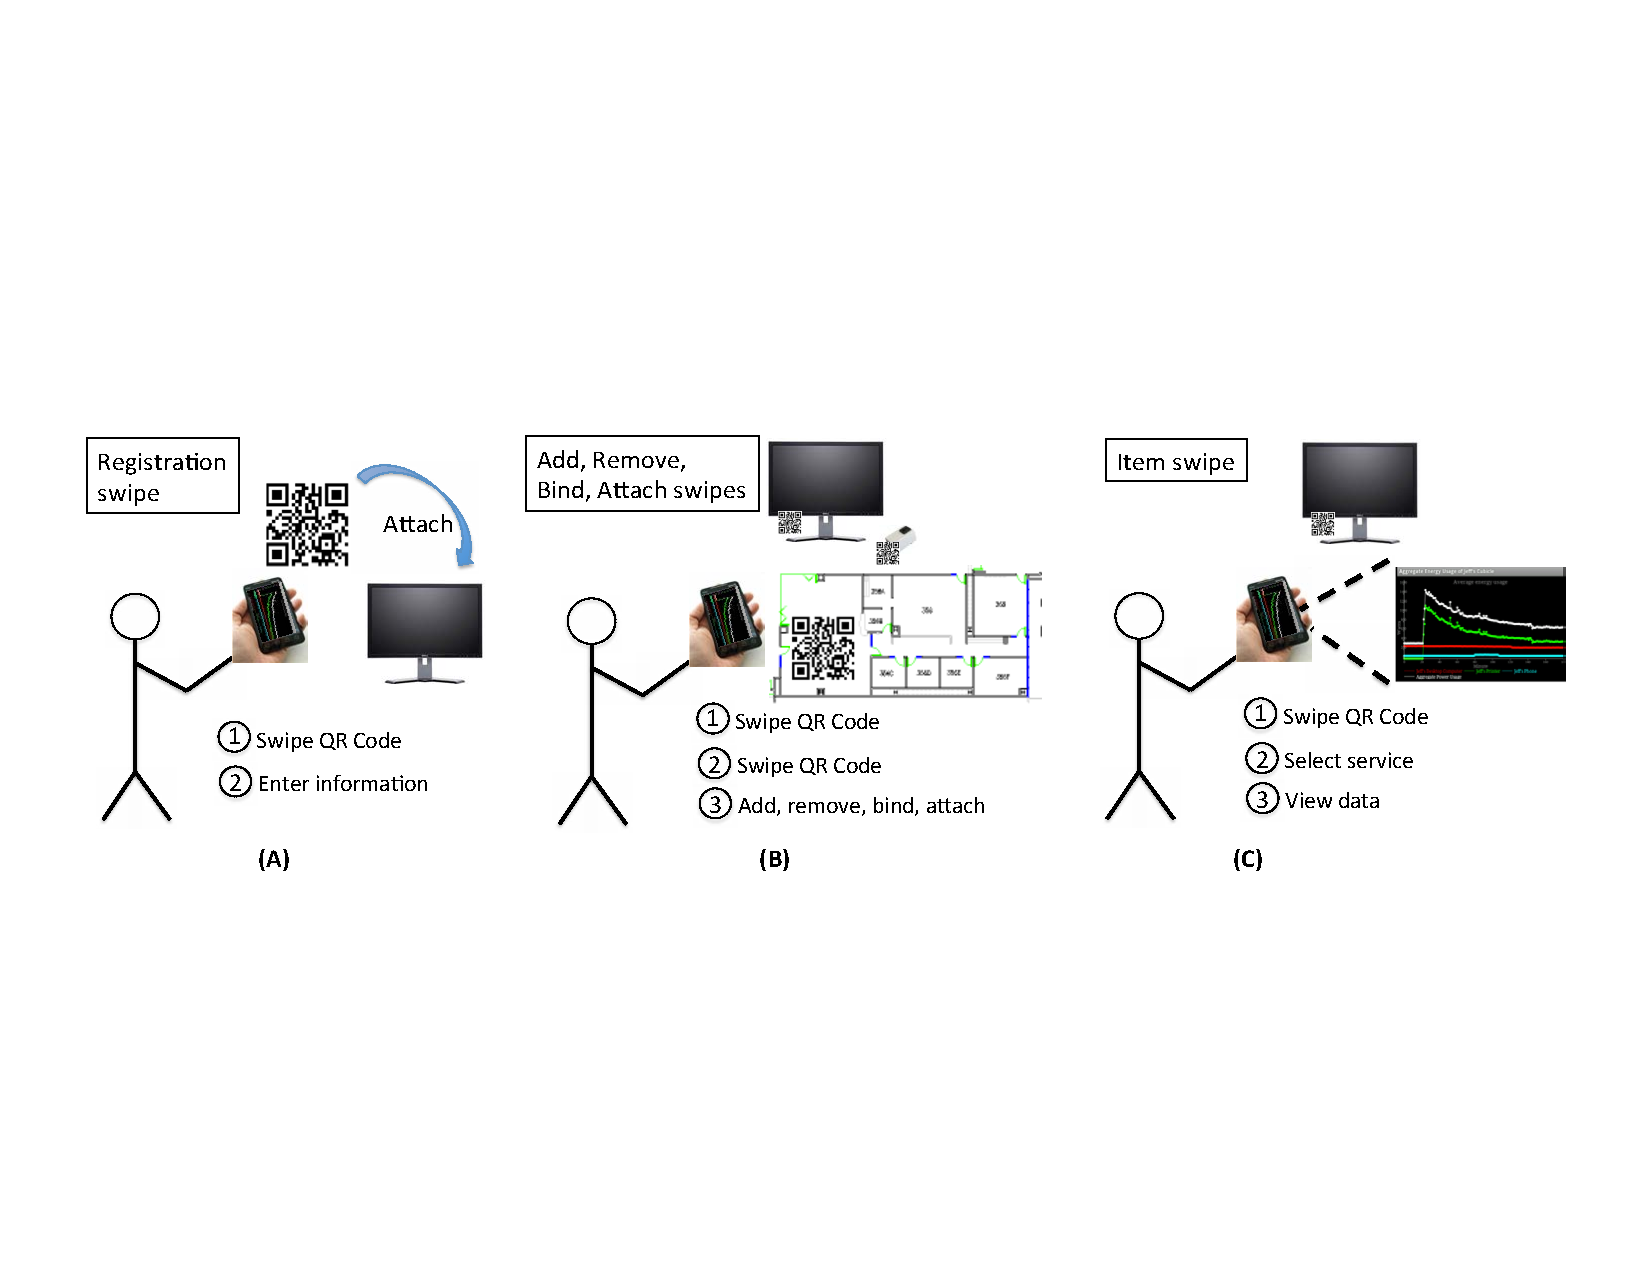
\includegraphics[width=\textwidth]{figs/swipes}
\caption{Gestures. Lorem Ipsum is simply dummy text of the printing and typesetting industry. Lorem Ipsum has 
been the industry's standard dummy text ever since the 1500s, when an unknown printer took a galley of 
type and scrambled it to make a type specimen book.  }
\label{fig:gestures}
\end{center}
\end{figure*}

\begin{figure}[htb!]
\begin{center}
\subfigure[Long QR Code.]{%
            \label{fig:qrcexfirst}
            
\includegraphics[scale=0.148]{figs/qrcexlong}
        }
\subfigure[Minimized QR Code.]{%
            \label{fig:qrcexsecond}
            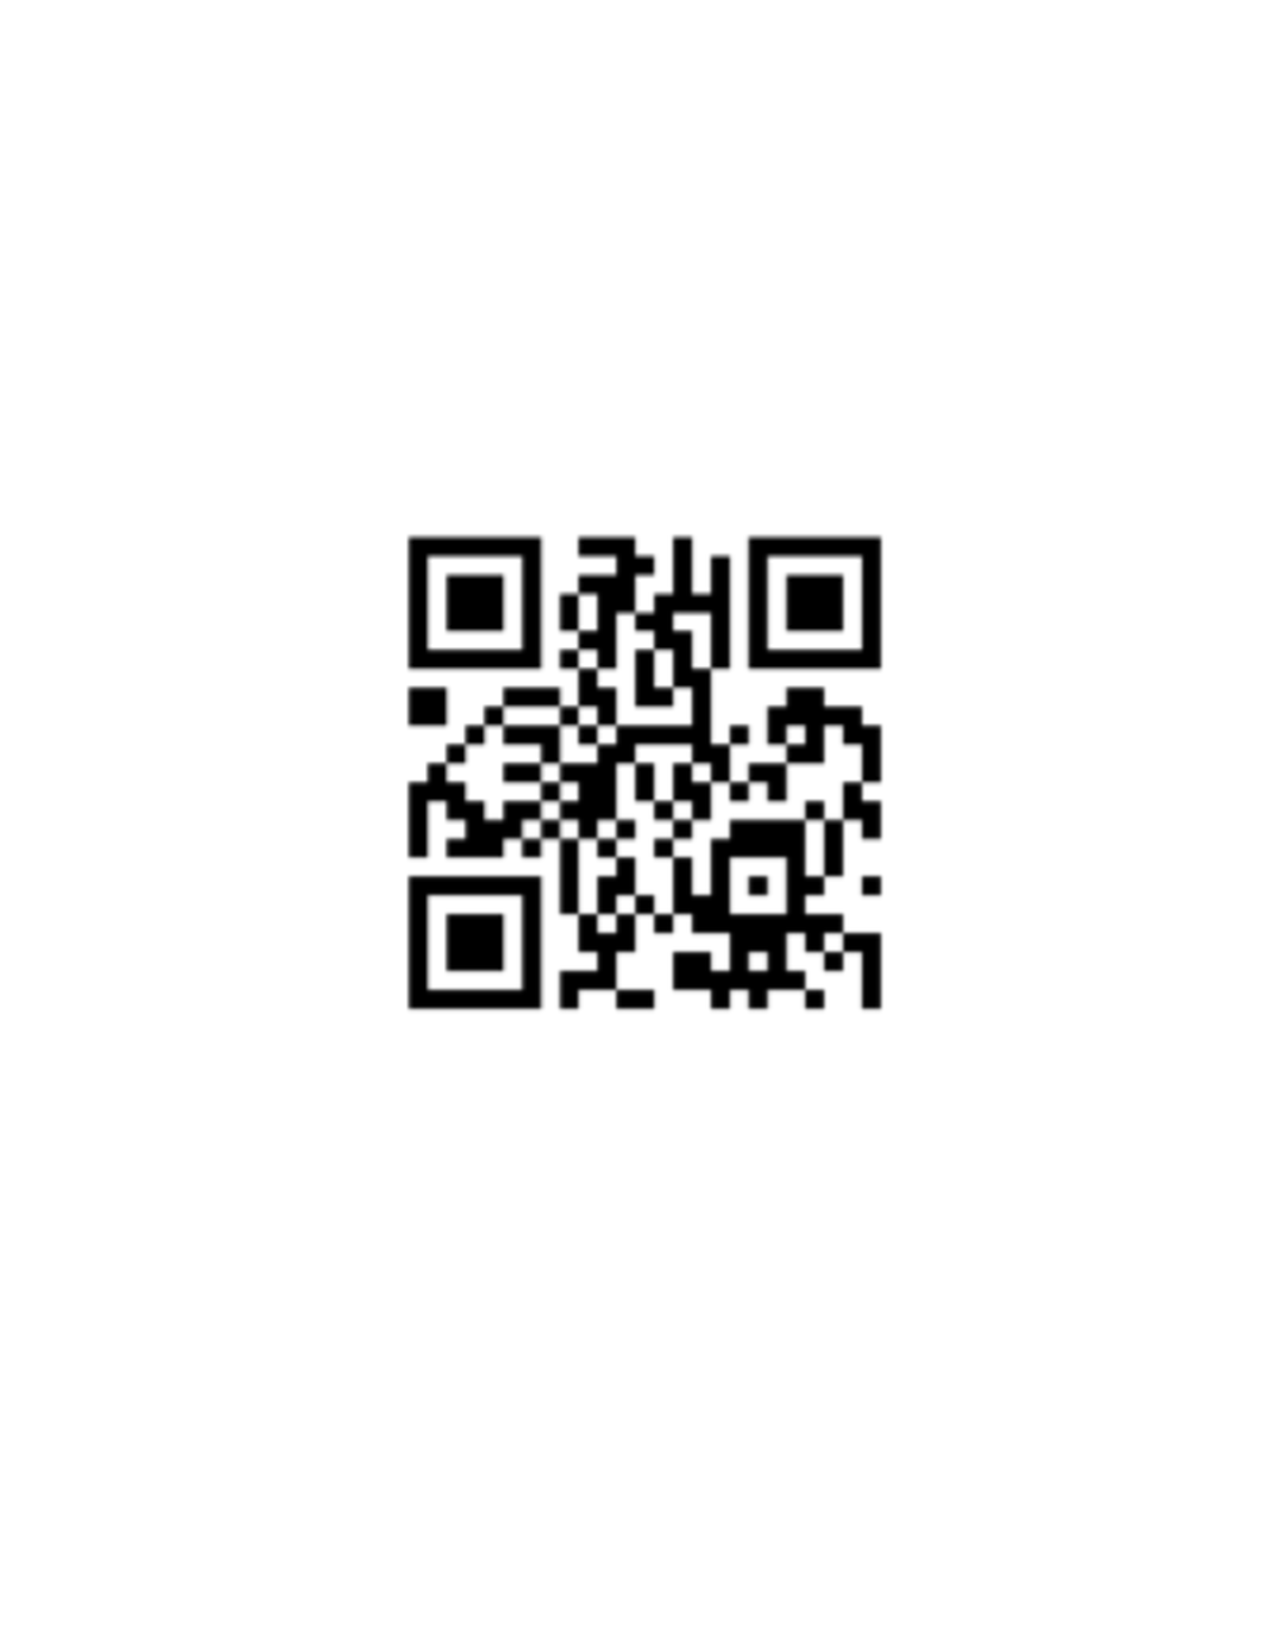
\includegraphics[scale=0.35]{figs/qrcex}
        }
\end{center}
\caption{
	The QR code on the left resolves to the same {\tt URL} at the right one, after resolution and
	redirection is complete. 
	The short label resolves to {\tt http://tinyurl.com/6235eyw}.  The second encodes about half
	the characters as the first.
	We used tinyUrl to reduce the QR code image complexity and scan time.
     }%
\label{fig:qrcexcomp}
\end{figure}

\begin{table}
\label{tab:qrscans}
\begin{center}
  \begin{tabular}{| r | c  c | }
    \hline
    			 & {\bf Average (sec) } & {\bf Variance (sec)} \\ \hline
    Short,light & 1.66 & 0.33 \\ \hline
    Short, dark & 2.08 & 0.35 \\ \hline
    Long, light & 2.26 & 0.71 \\ \hline
    Long, dark & 2.82 & 0.50 \\
    \hline
  \end{tabular}
\caption{Shows the time to scan a long QR code versus a short QR code in light and dark conditions (loosely defined).
Notice that short QR codes scan faster and with less variance that long ones.}
\end{center}

\end{table}

Table~\ref{tab:qrscans} shows the results of some simple scanning experiment between the two tags
shown above.  We scanned each QR code under light and dark lighting conditions, off the screen of my laptop.
Each experiment was run 10 times and the table shows the statistical
overview of the results. 
Clearly, scanning the simple QR code under well-lit conditions
performed the best.  The complex QR code under the same condition takes about 28-36\% longer to scan.
On a generic QR code scanner, as used here, there is a portion of the
scan time that is independent of the code complexity.  As these are
more heavily used, this is expected to be reduced substantially and
the difference is acquisition complexity will be even more pronounced.
Perhaps even more important is the variance.  Notice that the variance with the simple QR code is much smaller and
more stable under either condition.  In our experience, {\bf large variance in scan time is a major
problem for complex QR codes}.  Thus we decided to re-design our codes and push more information in the lookup
processes, as network access was more reliable than the focus of the camera on various mobile devices.
Tags are placed on all types of devices in all kinds of locations with varying degrees of lighting.
Simple QR codes are vital for widespread use.

The design choice forced us to examine others that were related.  Not being able to encode much information on 
our QR codes means we are more reliant on the network to provide the bulk of the information, to be very reliable,
and to be widespread enough that disconnection is not problematic.  Moreover, there are a number of clients
that can be used to access and display the information and the tag has to be meaningful for both.
In order to meet these criteria we (1) shrunk {\tt URL}'s using tinyURL~\cite{tinyurl} as a level of 
indirection and 
(2) designed two classes of applications: \emph{shallow} applications, and \emph{deep-inspection} applications.  Shallow
applications interact with the web-application directly while deep-inspection application use
the {\tt URL} of the web application to extract a unique identifier and provide deeper inspection
and update capabilities of the entity-relationship graph.

An example {\tt URL} we used in our deployment is {\tt http://tinyurl.com/6235eyw}.
When this is resolved, we get an empty response in the body, but we use the header to identify the QR code identifier 
that we associate with the item.  The response header looks as follows:
\begin{figure}[htb!]
\begin{center}
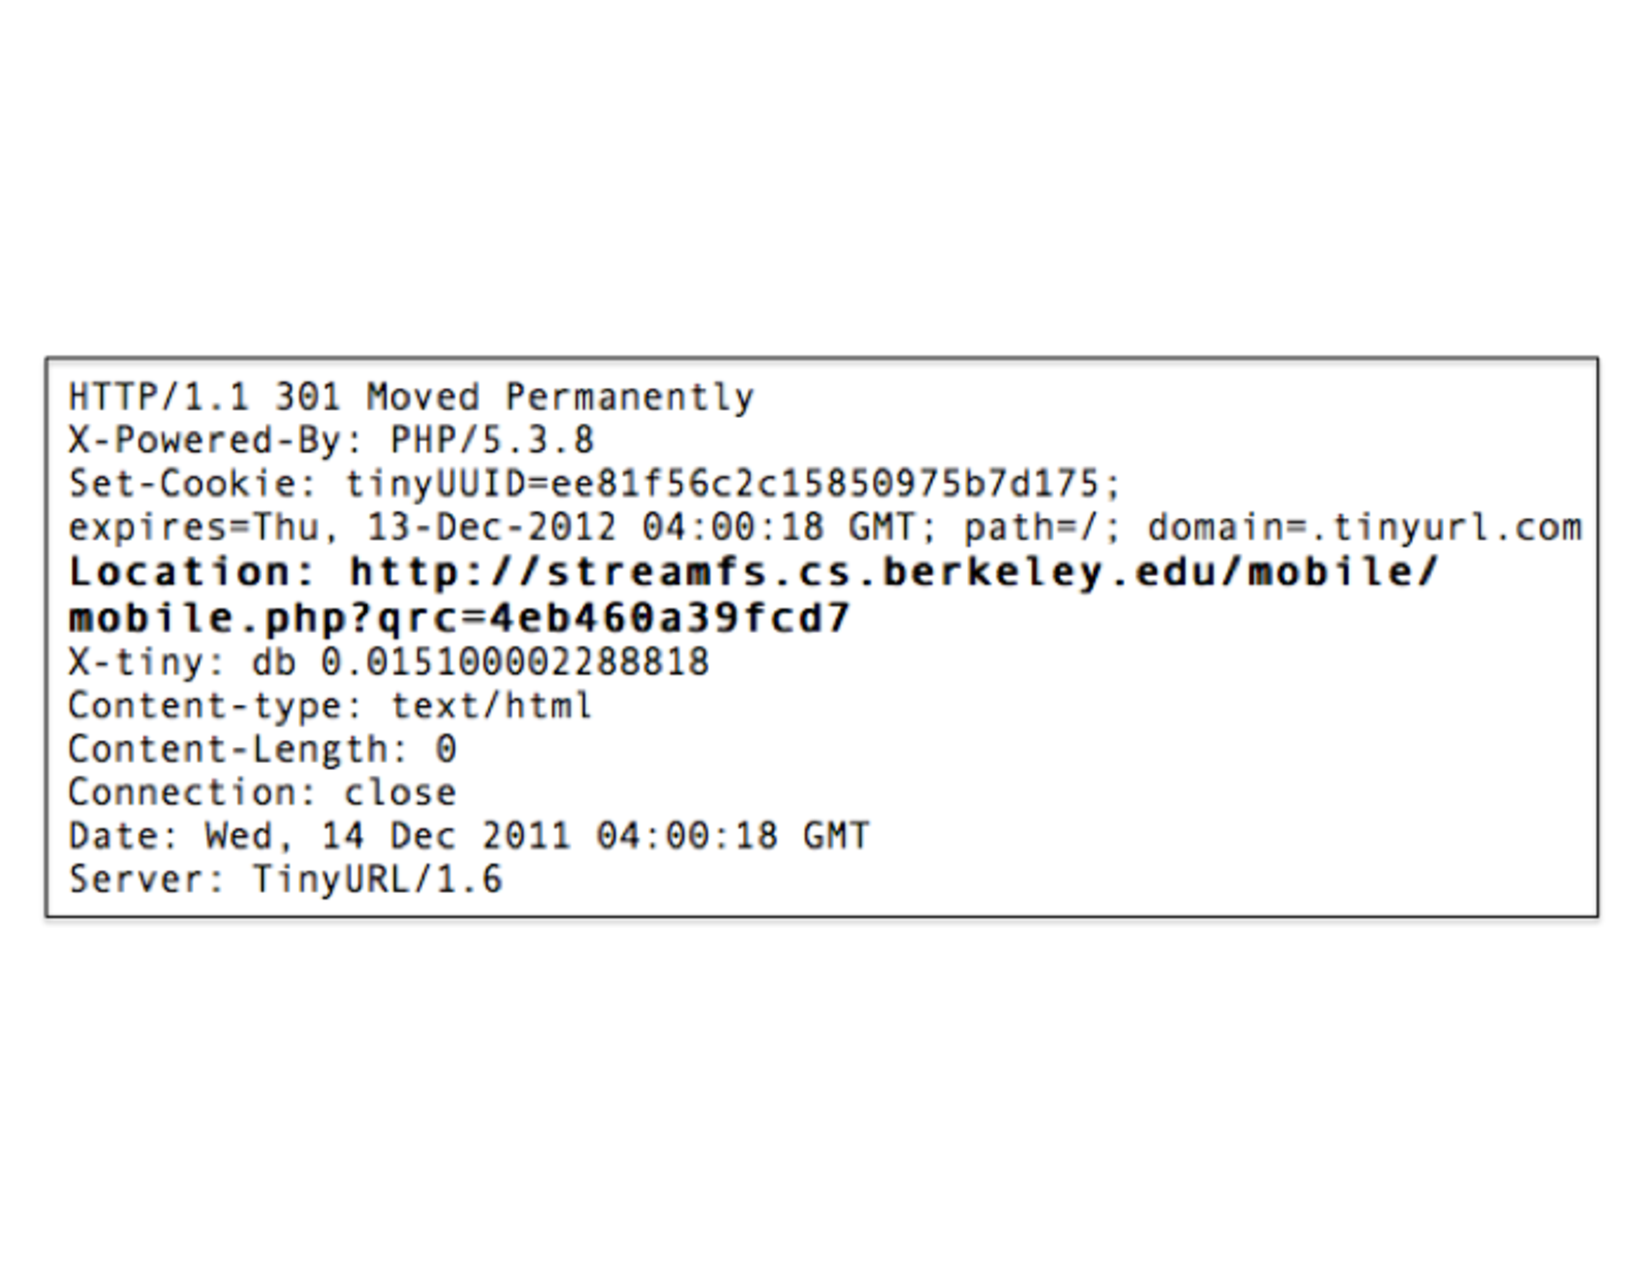
\includegraphics[scale=0.30]{figs/tinyurlhdr}
\caption{The header of the response from the {\tt tinyUrl} when resolving a QR code.  The `Location' attribute
is used to extract the unique identifier for the object this QR code tags.  It is also used to re-direct
users without the phone application to a meaningful web address for the object.}
\label{fig:tinyurlhdr}
\end{center}
\end{figure}

% It provides a web address for users to re-direct to and find information and various read-only services for the object.  However, because
% the {\tt URL} also contains a unqiue identifer \emph{qrc}, it can be used to provide for sophisticated services and capabilities.
% An example is the ability to change the virtual structure of inter-relationship between this object and other objects.  This
% is demonstrated in our energy auditing application discussed in detail in section~\ref{sec:eaudit}.
% Once items are tagged, they can be added and removed by swiping the tag and pressing the button for what you want to do with
% the item.  You also check into locations either explicit with a location-tag swipe or implicitly with an item swipe.

Notice the `Location' attribute in the header.  This is the location of the re-direct.  \emph{Shallow} applications
use the {\tt URL} directly.  The \emph{qrc} {\tt URL} is unqiue identifier for the item that this tag is attached to.
A shallow application can obtain mostly read-only service through our web applications.  For example, we'll see how
to get either item-specific data or item-aggregated data with respect to the user making the request (i.e. the total
energy consumed by \emph{my} devices).  \emph{Deep-inspection} applications are native to the phone, so we can do much
more with the tag.  Our energy auditing application allows you to related the item to other items by maintaining state of swipe
history.  This is more difficult with the web-applicaiton.  We can also use the tag and item information to couple it with
sensor information coming from sensors on the phone itself.  For example, we could determine the direction an object
is pointing by using the phone's directional sensor and negating their direction (i.e. phone is facing east, tag on item must
be facing west).






\subsection{Data management layer}

\subsection{Application layer}


\subsection{Disconnected operation}


\begin{figure}[htb!]
\begin{center}
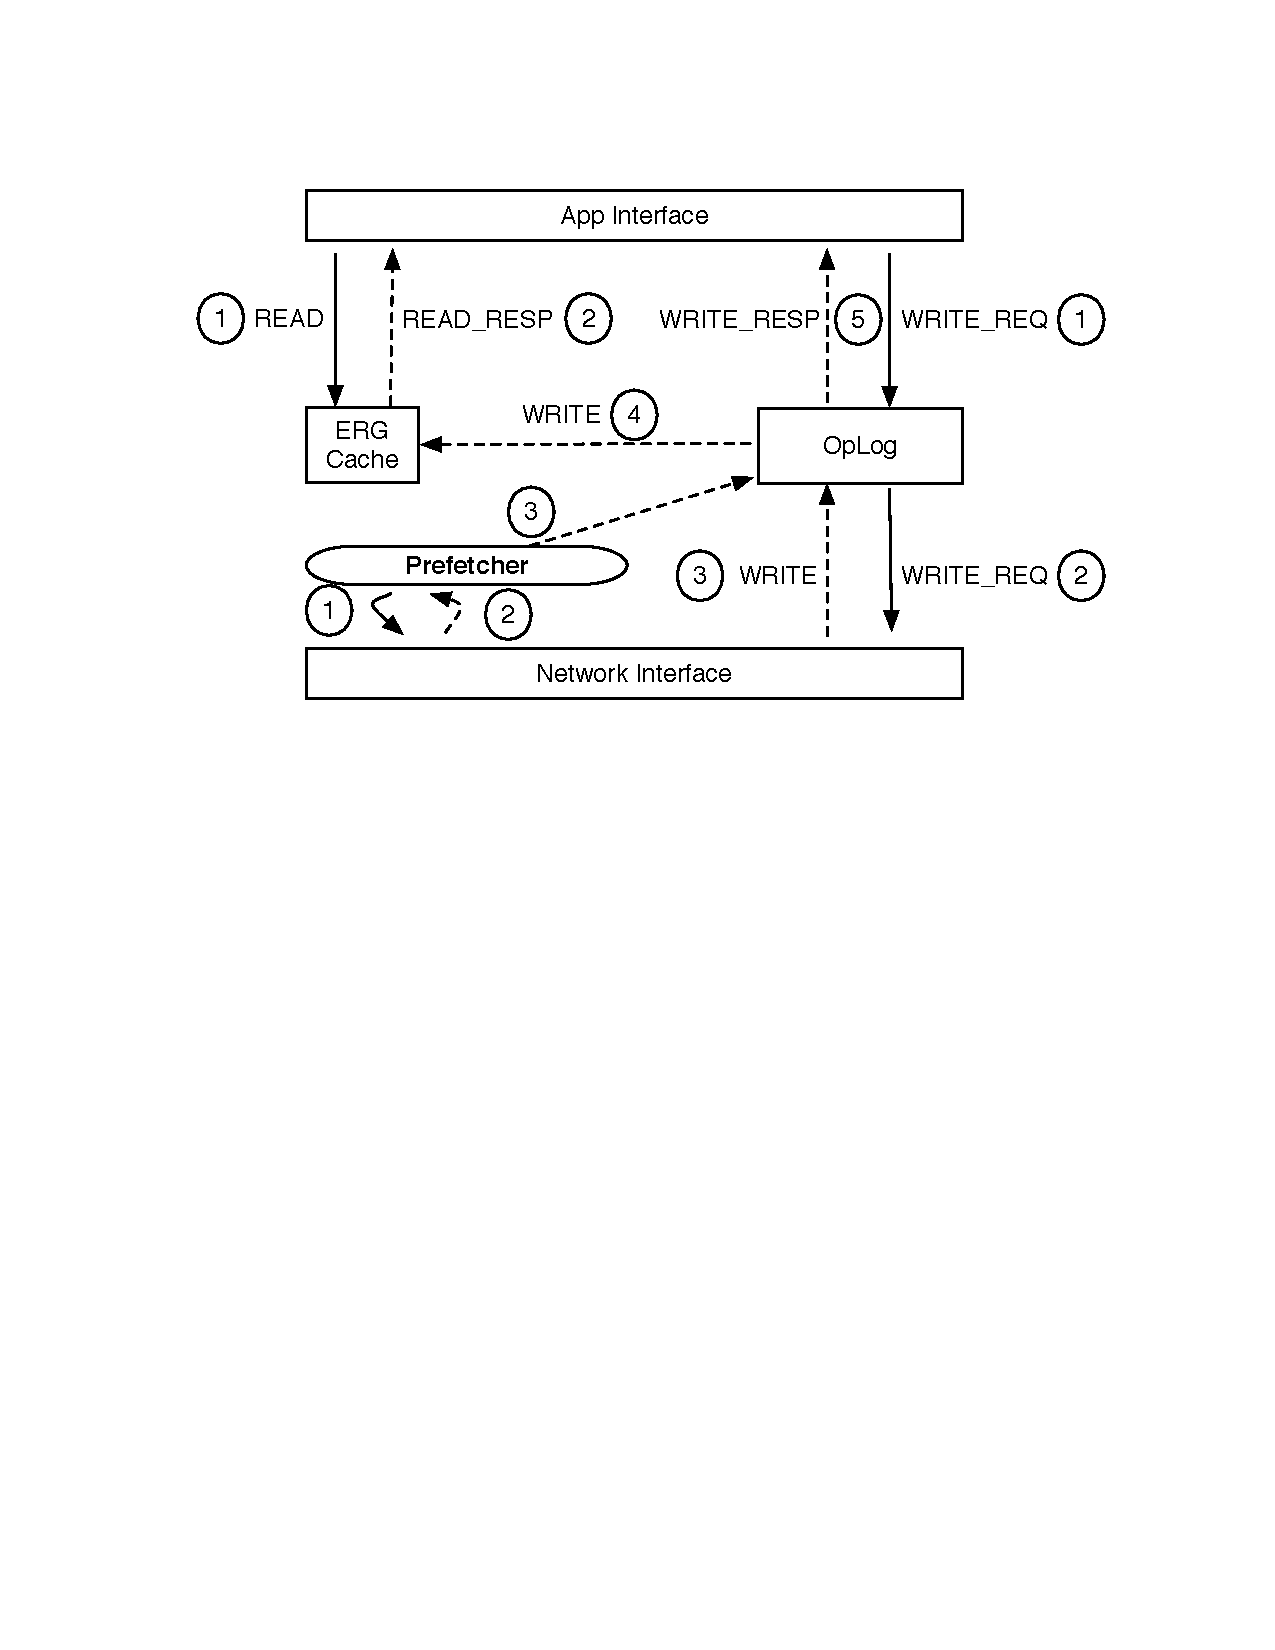
\includegraphics[scale=0.50]{figs/standard_interaction}
\caption{}
\label{fig:interactions}
\end{center}
\end{figure}


\subsection{Swiping gestures}
\label{sec:swipes}

\subsection{Tracking people and things}
There are three major components in our architecture: QR codes, mobile phones, and StreamFS.

How do we evaluate our ability to track people and things?
This is a description evaluation.  We need to describe how the pieces interact.  What will fall out of the description is our strong dependence on occupants/users to give us information about the state of the physical world.  It’ll also fall out that what allows these pieces to fit together is network infrastructure.



\subsection{consistency \& disconnected operations}

The ability to provide real-time analytics for physical data application is driven by 

The consistency and accuracy that we capture about the entities in the world and their relationships and associated metadata.
How those relationships/metadata inform our analytical operations.

Entities in the physical world can be difficult to capture and track over time.  Ideally we’d have a model of the world and the things in it and there would be a mechanism for tracking things that move.  We approximate this mechanism through the combination of QR codes, mobile phones, and people.  Items in the real-world are physically tagged with a QR code that serves as a reference for the “thing” in the physical world.  The mobile phone gives the person a ubiquitous QR code reader.  It also serves to provide the person with services associated with the physical world.

\subsection{Entity-Relationships}
The main aspect we want to capture is entity-relationships between the objects.  Entity relationships are captured through naming and interpreted by the EnergyLens application:

$/path/to/device\_or\_item$

$/path/to/qrc$

$/path/to/space$

$/path/to/taxonomy$

We essentially maintain for separate namespaces and we specify a relationship between them through links between these namespaces.  The relationship is also set by the type of item the path represents.  The types are item, meter, location, system\_device, category, and tag.\\

{\bf Bound-to}\\
When a meter is attached to an item and taking physical measurements associated with that device, we say that the meter is “bound-to” the device.

{\bf Attached-to}\\
When a meter/qr code/item is attached to another meter/qr code/item but NOT taking any physical measurements for that item, we say that the meter/item is “attached-to” the other meter/qr code/item.  QR codes should not be attached to each other and are not accepted by the EnergyLens application.

{\bf Inside-of}\\
When a meter/item is inside a location, we say that the meter/item is “inside-of” that location.

{\bf Type-of}\\
When an item is labeled by as a known, specific, type, we say that the item is a “type-of” thing specified by the its label.


\begin{figure}[htb!]
\begin{center}
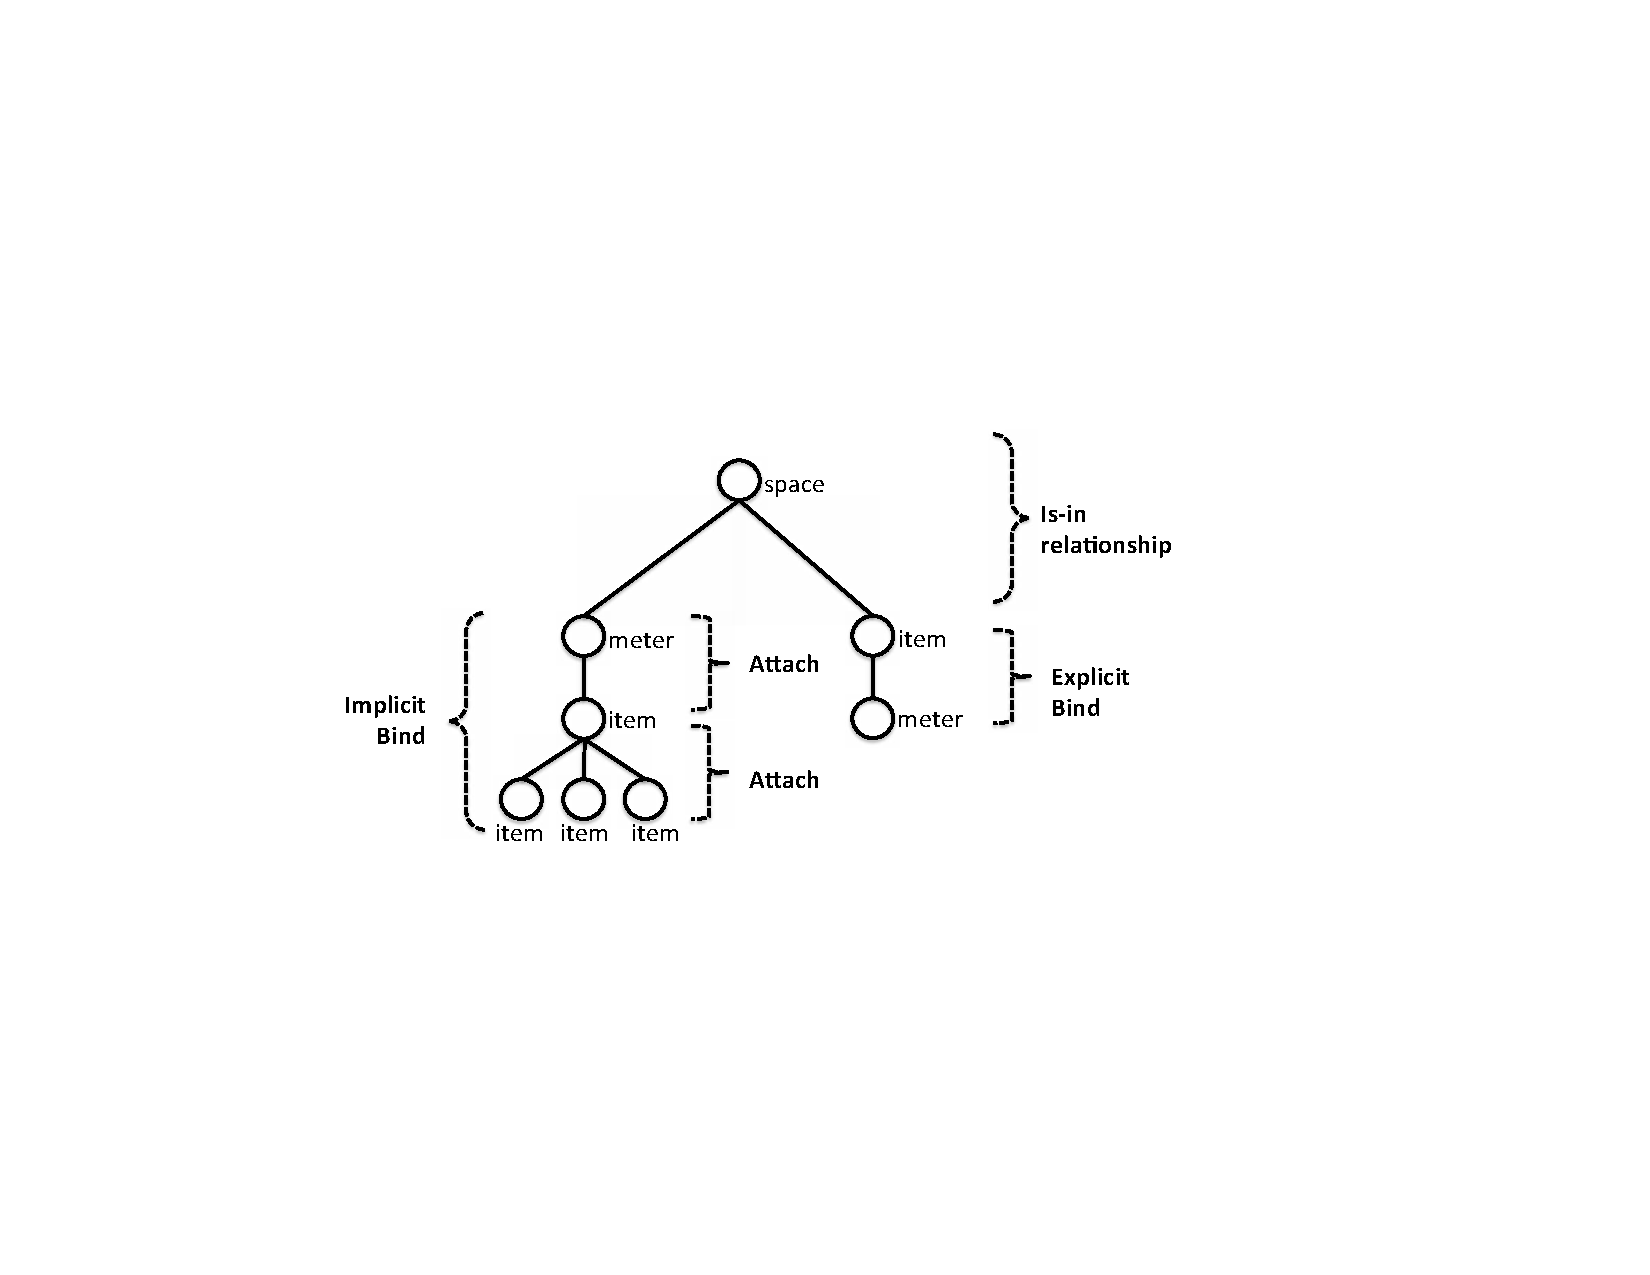
\includegraphics[scale=0.55]{figs/bindattachstructs}
\caption{This diagram shows the relationship capture between the objects and locations in the building for the 
energy audit application.  Children of a space node have an ``is-in'' relationship with the space.  An item
with another item as a child have a ``attached'' relationship and meters attached to items are bound to each other.
Note, this is a \emph{subset} of the relationship diagrams generated across our three applications.}
\label{fig:attachandbind}
\end{center}
\end{figure}

\subsection{Managing consistency while disconnected}

\subsubsection{Caching}
Although network connectivity is theoretically ubiquitous, in practice, this is not always the case.  In order to enable updates while disconnection we need to cache as much of the relevant deployment state as possible.

\subsubsection{Pre-fetching \& The state-change stream}
We should pre-fetch, as the tags inform us about what the user might access next.  What are some things to pre-fetch?  All the paths from the current root to the leaves.  We should also fetch the object associated with each file and for streams, we should fetch 1 hours’ worth of data.  In most cases this means fetching about 200-400 KB of data.

\begin{figure}[htb!]
\begin{center}
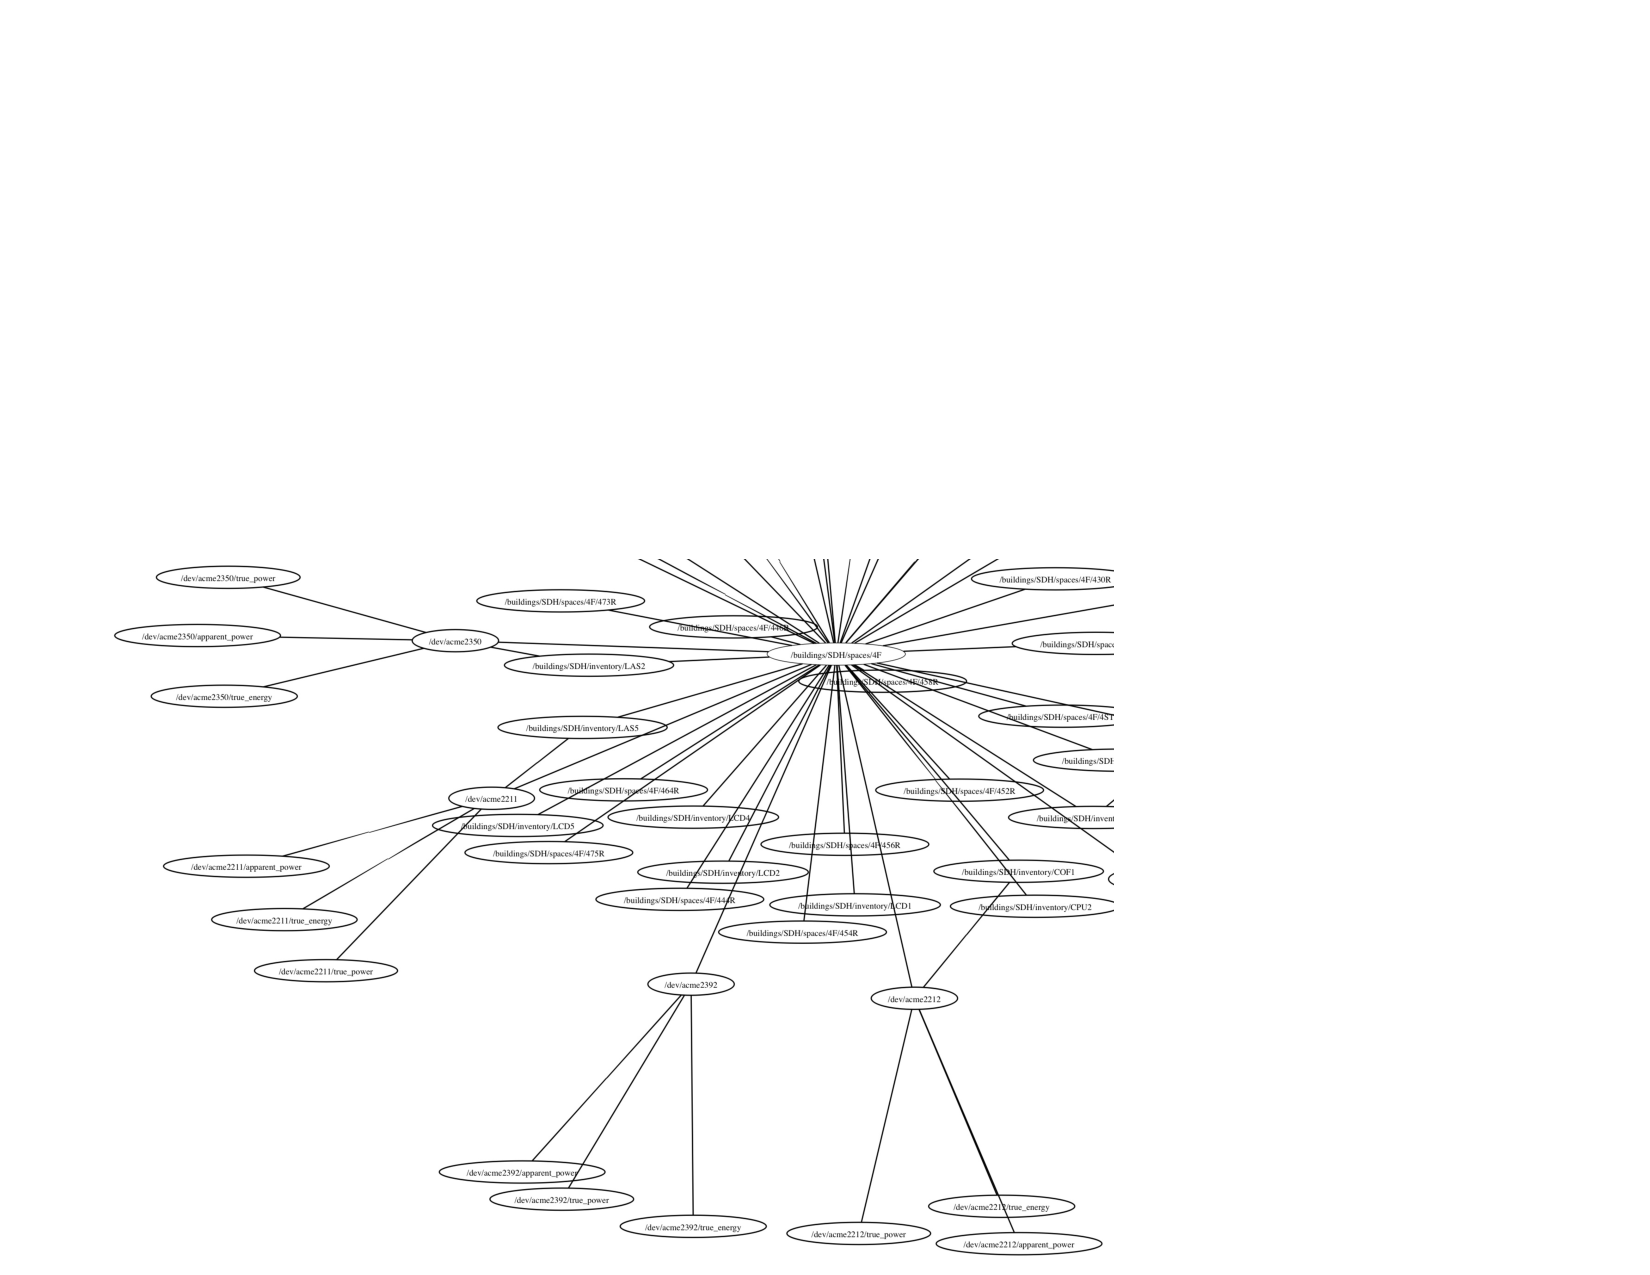
\includegraphics[scale=0.55]{figs/SDH_4F_ERG_closeup}
\caption{A portion of the prefetched entities on the a single floor in our building.  This shows a snapshot of the entity-relationship
graph for that floor.  Each node, link, and associated content is prefetched when the user swipes the floor
tag or anything on that floor.}
\label{fig:sdh_4f_erg}
\end{center}
\end{figure}

\subsection{Conflict resolution}
All transactions are processed in timestamp order, to some rough approximation of the time that the transaction would have been committed.  When a transaction with an earlier timestamp than the last committed transaction is offered, the EnergyLens transaction manager checks if the current transaction conflicts with any previously committed transaction.  This is done by checking if the files that are touched overlap with a transaction that touches the same files and has a transaction timestamp that’s later than the current transaction being offered.  If so the transaction manager rolls back the state of StreamFS, only for the affected files, back to the last transaction before the last commit.  It then commits the offered transaction, adds it to the transaction log, and replays the transaction that was rolled back.  If the operations of the replayed transaction are no longer valid, the transaction fails silently.  Failing silently is acceptable in this context because we want to capture the latest state of the world.  By rejecting the transaction, we are assuming that it was based on false assumptions about the state of the world.  We believe this assumption to be true in most cases.


\subsection{Maintaining, representing, and using physical state and inter-relationships}
In order to provide relevant services, we need to capture the state of the physical environment within the building.  By “relevant”, we mean based on context and inter-relationships.  What are “the relevant services” we’re talking about?

\begin{itemize}
\item Energy analytics on the physical world.
\item How much does this floor consume?
\item What fraction of that is going to the various energy-related categories?  plug-load, hvac, lighting.
\item Personalized energy analytics.
\item Access the the control interface for the physical world.
\end{itemize}

\subsubsection{General approach}
Our approach is to abstractly represents things in the environment as logical entities and to capture their inter-relationships through an entity-relationship graph.  We use the entity relationships to track where objects and things are in the environment, which helps us maintain a more consistent view of the world.  We also use  it to inform our analytical approach and our choice of services to display.

\subsubsection{Consistency management}
Connecting the various components requires ubiquitous connectivity.  Although connectivity is available through the building and the access-point deployment is engineered to minimize dead spots, disconnections still occur (timeout, dead-spots, unsuccessful handoffs).  So, we need to design the system to deal disconnect operation.

Evaluation will be of a protocol description and design rationale described in detail here.
What’s the evaluation exactly?

\begin{enumerate}
\item Time to download the associated contextual information from StreamFS: files, metadata information, data**
\item Conflict resolution examples**
\item Optimizations: Pre-fetching measurements**
\end{enumerate}

\subsection{Real-time analytics}
Discussion.  What to measure here?  Perhaps we discuss the relevant real-time analytics we run?  Will there be space?  For buildsys, include a half page talking about some of the analytics.
% Pub/sub architecture
% time decoupling
% variable time-decoupling achieved through the datastore as a buffer
% synchronization decoupling
% Either the publisher or subscriber run asynchronously.
% space decoupling
% The subscriber doesn’t have an explicit reference to the publisher.
% Programming model for real-time data
% Naming/tagging streams
% Dealing with dynamism through tagging
% Built-in functions for physical data
% heat modeling
% electrical modeling
% mathematical modeling

% Security and privacy
% Discussion.  Various topics related to StreamFS here.  Also some topics related to managing security in StreamFS for doing control.  Include another half page, perhaps.


% * Experiment that we need to run.\\
% ** Code that needs to be written and experiment that needs to be run
\section{Evaluation}
\label{sec:eval}
In this section we measure prefetch download times and discuss strategies for providing scalability.  We also
look at the transaction manager and evaluate conflict resolution times.

% \begin{figure}[htb!]
% \begin{center}
% 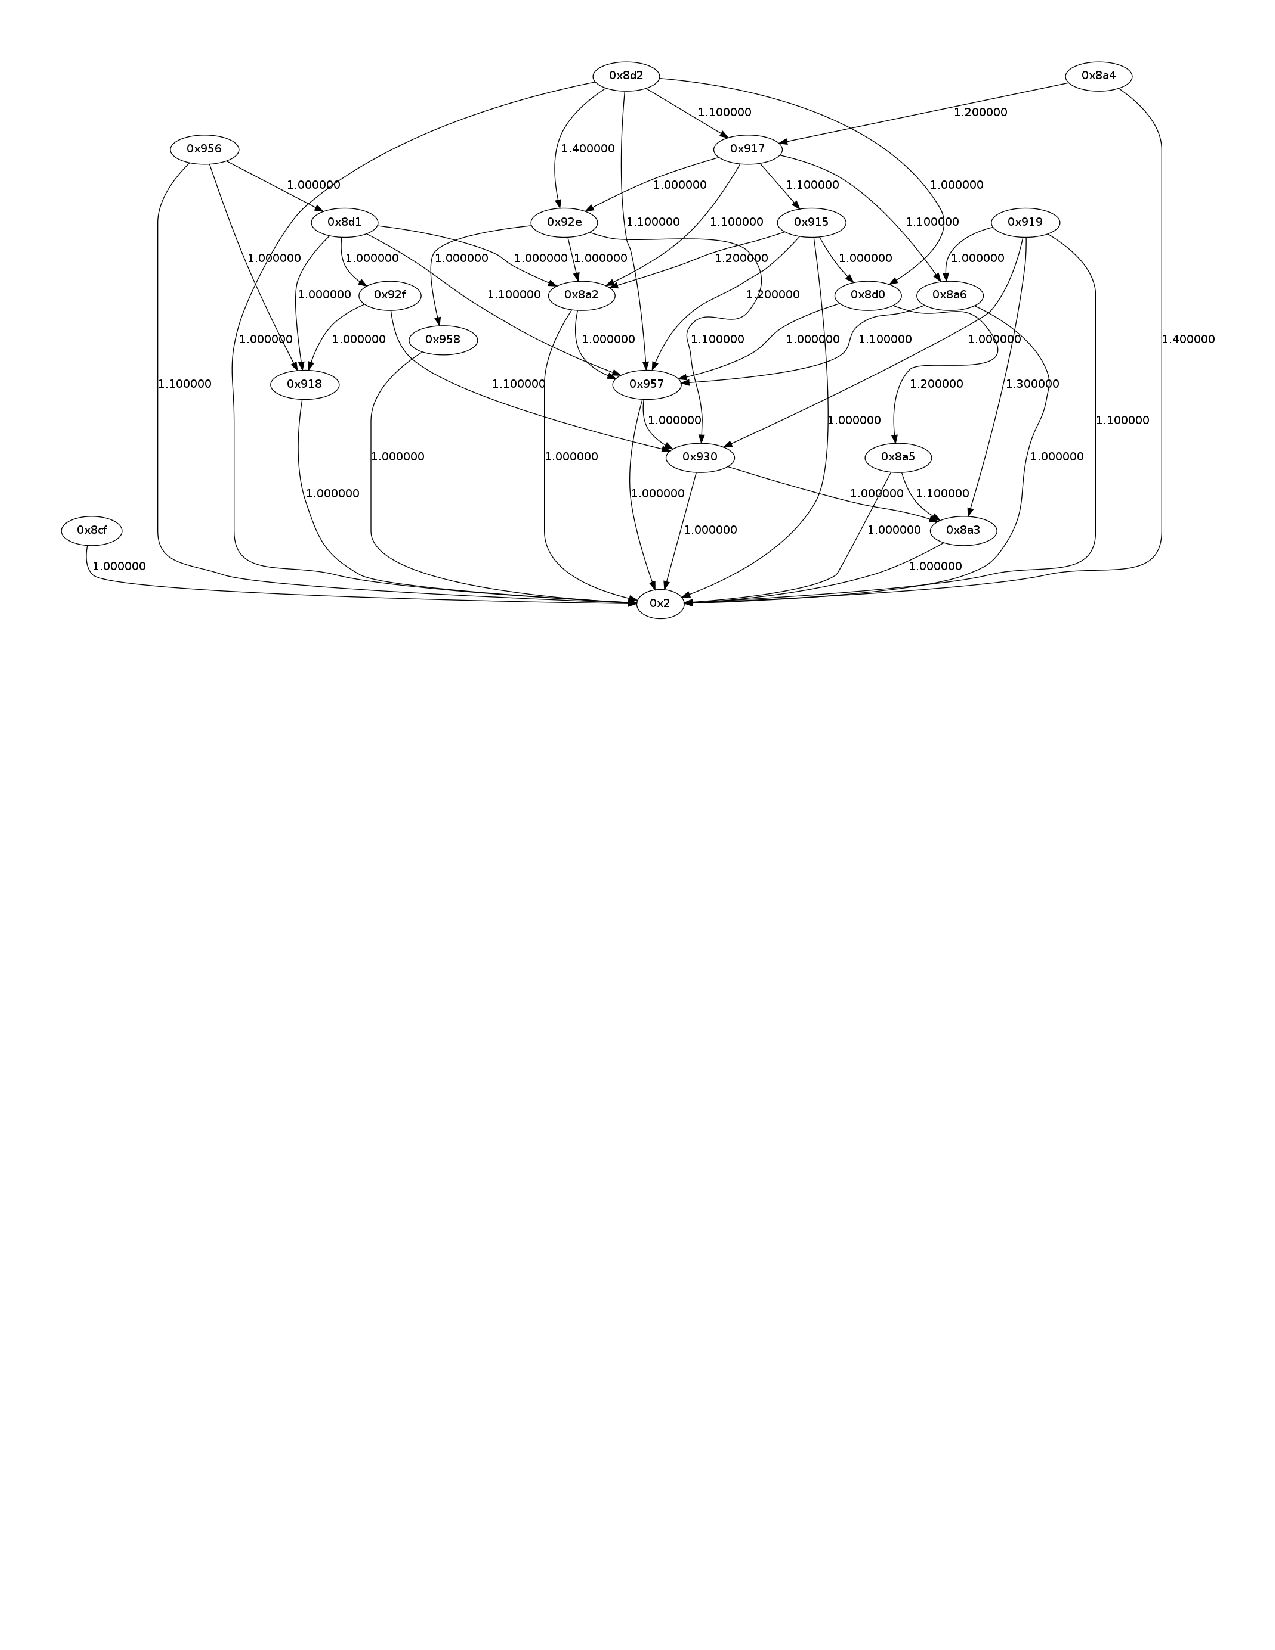
\includegraphics[scale=0.4]{figs/acmenetwork_SDH_4F}
% \caption{}
% \label{fig:acmenetwork_SDH_4F}
% \end{center}
% \end{figure}


\subsection{Prefetching}
Prefetching occurs when a user enters a new floors, as detected by a floor scan or an item
scan.  Table~\ref{tab:prefetchtimes} shows that the prefetch times scale linearly with the number of
items (and data) to prefetch.  Each node holds approximate 100 bytes or information and for
a 20-node deployment of power meters, producing 100 bytes of data per stream (3) every 20 seconds, we fetch 
approximately 1 MB of data.

These prefetch times are non-trivial to deal with, especially since they cause the phone application to slow down
until the data received and loaded into the local cache.  The overhead is dominated by the query in StreamFS that 
constructs the entire sub graph to send to the application.  For future work,  we are will implement a
callback facility and pass the application a reference to it.  The app can then periodically check back until
the query completes and the data is ready to be downloaded.  We can also include partial responses to the query
in the prefetch loop response.  This also allows user to continue using the application without any frustrating waits.

% \subsection{Log dump measurements}
\begin{table}
\begin{center}
  \begin{tabular}{| r | c  c | }
    \hline
    {\bf No. nodes } & {\bf Fetch time (sec) } & {\bf Std. Error (sec)} \\ \hline
    1 & 0.8902 & 0.0756 \\ \hline
    10 & 5.7342 & 1.7087 \\ \hline
    100 & 52.3145 & 14.1146 \\ 
    \hline
  \end{tabular}
\caption{Shows the time to fetch nodes based on the size of the fetch.  The fetch time
increased linearly with the number of nodes.  Caching maintain fetch time near
that of fetching a single node.  A callback is used when cache is invalidated.}
\label{tab:prefetchtimes}
\end{center}
\end{table}


\subsection{Log replay latency}
Table~\ref{tab:optimes} shows the  operation that the transaction manager calls on the StreamFS server.
Log replay and transaction processing is entirely dependent on the time to execute these operations on StreamFS.
There are two types of transactions, a \emph{move}, a \emph{un/bind}, \emph{un/attach}.  A move is a combination
of a `delete' and a `create link', a bind is a `create link' and an `update tags', an unbind and unattach is a
`delete' and `undate tag'.  The transaction latency is the sum of these operations.  By far the most expensive
operation is a `create node' operation.  This occurs when a user adds a new item/space/person to the graph.
The time to apply the operation scale linearly with the size of the logs.  

All logs dumps are processed sequentially.  However, for future work we look to parallelize processing into
parallel processes updating different portions of the graph.  For example, log updates rooted at different floors
could occur simultaneously.




% The global transaction manager implements three main high-level operations -- rollback, apply, and replay.  Our current implementation
% is limited by the time is takes to perform an operation on StreamFS.  Table~\ref{tab:optimes} shows the three 
% main operation that the transaction manager needs to do on the server.
% % Maybe we include another table that talks about the trace we ran through and the conflict times, etc.

% Usually rollbacks consist of \emph{delete} operation and applies consist of \emph{creates}.  In a worst-cases analysis
% of performance we expect the total conflict resolution time to be roughly bounded by
% $rollback\_time + apply\_time + replay\_time$, since $replay\_time=3 X rollback\_time$ and apply\_time is negligible, 
% the total time is approximately $4 X rollback\_time$.  Therefore the overhead is driven by how many new links were created
% that have to be deleted and then re-created.  As an optimization, we limit the scope of a rollback.  The naive
% approach is to blindly undo all operations up to a certain time.  However, we can use the location of the node
% in the ERG to limit the conflict-scope to a sub graph, rather than the entire graph.  The simplest approach is to check if the operation
% on a node either shares an immediate parent with the node that will have an operation undone on it or it the operation
% is on the same node.  By limiting conflict-scope we minimize the number of operation that get execute and, hence, minimize the 
% cost of resolution.



\begin{table}
\begin{center}
  \begin{tabular}{| l | c  c | }
    \hline
    {\bf Operation } & {\bf Avg. exec. time (ms) } &\\ \hline
    fetch & 250 &\\ \hline
    delete & 326  &\\ \hline
    update tags & 267  &\\ \hline
    create link & 250  &\\ \hline
    create node & 1036  &\\ 
    \hline
  \end{tabular}
\caption{Average operation execution time in StreamFS.}
\label{tab:optimes}
\end{center}
\end{table}

% \begin{itemize}
% \item Forwarding
% \item Conflict resolution
% \end{itemize}




% The main driver for the EnergyLens work is to explore the fundamental challenges related to:

% \begin{enumerate}
% \item Tracking people and objects.
% 	\begin{itemize}
% 	\item Through local crowd-sourcing of the tasks to building occupants
% 	\end{itemize}
% \item Maintaining consistency between the relationship between physical items and the entity-relationship graph that represents it.
% \item Providing real-time statistics, information, and processing of energy data related to the building environment.

% 	\begin{itemize}
% 	\item With respect to the occupants
% 	\item with respect to spaces
% 	\item Maintaining security and privacy
% 		\begin{itemize}
% 		\item specifically with respect to personal data and control
% 		\end{itemize}
% 	\end{itemize}

% \end{enumerate}


\subsection{Limitations}
EMD is useful for finding underlying behavioral relationships between traces of sensor data.  However,
when we set the timescales smaller than a day, the results were not as strong.
The trace has to be long enough to capture the trend.  For this data set, the underlying
trend is daily, therefore it requires there to be a significant number of samples over many days.
%  to
% for this method to be effective.
Although this was a limitation for this dataset, it really depends on the underlying phenomenon that
the sensors are measuring.  Its underlying trend is ultimately what EMD will be able to separate
from the intrinsic modes of the underlying signal.

\subsection{Discussion}
EMD allows us to effectively identify fundamental relationships between sensor traces.
% Using EMD to find fundamental relationships between sensor traces effectively identifies intrinsically
% related behavioral relationships.
% was quite promising for building
% up models of correlated usage.  
We believe that identifying meaningful usage-correlation patterns can help reduce oversights
by the occupants and faults that lead to energy waste.  A direct application of this is the identification
of simultaneous heating and cooling~\cite{simheatcool}.  Simultaneous heating and cooling is when heating
and cooling system either compete with one another or compete with the incoming air from outside and is
a cause for major energy waste in building~\cite{simheatcool}.  The longer it goes undetected,
the more waste there is.  However, it is very difficult to identify since the occupants do not notice
changes in temperature.  Our analysis can be used to build a correlation model between the outside
heating cooling temperature, the cooling coil temperature, and the outside air vent position.  If their behavior
is not correlated as expect, an alarm should be raised.

We can also apply it to other usage scenarios.  In our traces, for example, we found an instance where the pump
was on, but the lights were off.  The two are typically correlated, however, in this case they were not.
The air conditioning was pumping cool air into a room without occupants.
With our approach this could have been identified and corrected.  In future work, we intend to
package our solution to serve these kinds of applications.

% EMD works perfectly although the weekly pattern of the data is altered the last analyzed week.

% EMD inherently finds the interesting time scales.

% number of zero crossing = mean frequency/time scale:
%   TODO give the time scale for each IMF.


\section{Conclusion}
% what is our problem

% what we did

% contributions and main results

% future work


This paper set out to examine the underlying relationship between sensor traces to find interesting correlations
in use.  We used data from a large deployment of sensors in a building and found that direct correlation analysis on the raw
traces was not discriminatory enough to find interesting relationships.  Upon closer inspection, we noticed that
the underlying trend was dominating the correlation calculation.  In order to extract meaningful behavior this trend has
to be removed.  We concluded that empirical mode decomposition is a helpful analytical tool for de-trending 
non-linear, non-stationary data; inherent attributes contained by our traces.

We re-ran our analysis on the same traces, except we correlated the IMF outputs of the EMD operation on each of the traces and found that the pump was closely related to the lights in the same room served by the pump and
uncorrelated with a pump on the same floor serving a different room.  In order to corroborate the applicability
of our approach, we compared the pump trace with \emph{all} 674 sensor traces and found a strong correlation
between the relative spatial position of the sensors and their IMF correlations.  The most correlated IMFs were 
serving the same
area in the building.  As we relax the admittance criteria we find that the spatial correlation expands radially from
the main location served by the reference trace.

We plan to examine the use of this method in applications that help discovery changes in underlying relationships over time
in order to identify opportunities for savings in buildings.  We will use it to build inter-device correlation models
and use these models to establish ``normal'', ``abnormal'' usage patterns.  We hope to take it a step further and include a
supervised learning approach to distinguish between ``efficient'' and ``inefficient'' usage patterns as well.











\chapter{Lessons Learned and Future Work}
\chapter{Conclusion}

% \appendix
% \chapter{More Monticello Candidates}

\printbibliography

\end{document}
